\documentclass[11pt, fleqn]{article}
\usepackage[english]{babel}
\usepackage[utf8]{inputenc}
\usepackage[T1]{fontenc}
\usepackage{todonotes}
\usepackage{amssymb}
\usepackage{verbatim}
\usepackage{color}
\usepackage[lmargin=1.1in,rmargin=1.1in,bottom=1.3in,top=1.3in,twoside=False]{geometry}

\usepackage{relsize,xspace}
 \usepackage{xcolor}
 \usepackage{mathtools}

\usepackage{microtype}
\usepackage{amsmath}
\usepackage{amssymb}
\usepackage{amsfonts}
\usepackage{stmaryrd}
\usepackage{tikz}
\usepackage{bm}
\usepackage{tikz}

\definecolor{light-blue}{rgb}{0.2,0.4,0.9}
\usepackage[ocgcolorlinks, allcolors={light-blue}]{hyperref}
% \definecolor{light-blue}{rgb}{0.7,0.8,1}
% \usepackage[allbordercolors={light-blue},pdfborderstyle={/S/U/W 0.8}]{hyperref}

\usepackage[amsmath,thmmarks,hyperref]{ntheorem}
\usepackage{cleveref}

\crefformat{page}{#2page~#1#3}%
\Crefformat{page}{#2Page~#1#3}%
\crefformat{equation}{#2(#1)#3}%
\Crefformat{equation}{#2(#1)#3}%
\crefformat{figure}{#2Figure~#1#3}%
\Crefformat{figure}{#2Figure~#1#3}%
\crefformat{section}{#2Section~#1#3}
\Crefformat{section}{#2Section~#1#3}
\crefformat{chapter}{#2Chapter~#1#3}
\Crefformat{chapter}{#2Chapter~#1#3}
\crefformat{chapter*}{#2Chapter~#1#3}
\Crefformat{chapter*}{#2Chapter~#1#3}
\crefformat{part}{#2Part~#1#3}
\Crefformat{part}{#2Part~#1#3}
\crefformat{enumi}{#2(#1)#3}
\Crefformat{enumi}{#2(#1)#3}

\usepackage{latexsym}

% BEGIN ntheorem configuration

\theoremnumbering{arabic}
\theoremstyle{plain}
\theoremsymbol{}
\theorembodyfont{\itshape}
\theoremheaderfont{\normalfont\bfseries}
\theoremseparator{}

\newtheorem{theorem}{Theorem}[section]
\crefformat{theorem}{#2Theorem~#1#3}
\Crefformat{theorem}{#2Theorem~#1#3}

\newcommand{\newtheoremwithcrefformat}[2]{%
  \newtheorem{#1}[theorem]{#2}%
  \crefformat{#1}{##2\MakeUppercase#1~##1##3}%
  \Crefformat{#1}{##2\MakeUppercase#1~##1##3}%
}

\newtheoremwithcrefformat{proposition}{Proposition}
\newtheoremwithcrefformat{observation}{Observation}
\newtheoremwithcrefformat{lemma}{Lemma}
\newtheoremwithcrefformat{conjecture}{Conjecture}
\newtheoremwithcrefformat{corollary}{Corollary}
\theorembodyfont{\upshape}
\newtheoremwithcrefformat{example}{Example}
\newtheoremwithcrefformat{remark}{Remark}
\newtheoremwithcrefformat{claim}{Claim}

\theoremsymbol{\ensuremath{□}}
\newtheoremwithcrefformat{definition}{Definition}

\theoremstyle{nonumberplain}
\theoremheaderfont{\scshape}
\theorembodyfont{\normalfont}
\theoremsymbol{\ensuremath{\square}}
\newtheorem{proof}{Proof.}

% END ntheorem configuration


\setlength{\parskip}{0.3cm}
\setlength{\parindent}{0cm}
\setlength{\mathindent}{1.5cm}

\newcommand{\wcol}{\mathrm{wcol}}
\newcommand{\col}{\mathrm{col}}
\newcommand{\adm}{\mathrm{adm}}
\newcommand{\Wreach}{\mathrm{WReach}}
\newcommand{\Sreach}{\mathrm{SReach}}
\newcommand{\wcolorder}{\sqsubseteq}
\newcommand{\Oof}{\mathcal{O}}
\newcommand{\CCC}{\mathcal{C}}
\newcommand{\DDD}{\mathcal{D}}
\newcommand{\Vv}{\mathcal{V}}
\newcommand{\fv}{\textrm{FV}}
\newcommand{\embed}{\hookrightarrow}

\newcommand{\ie}{i.e.\@ }
\newcommand{\N}{\mathbb{N}}
\newcommand{\R}{\mathbb{R}}
\newcommand{\Rbar}{\overline{\R}}
\newcommand{\tup}[1]{\overline{#1}}
\renewcommand{\phi}{\varphi}
\newcommand{\strA}{\mathfrak{A}}
\newcommand{\strB}{\mathfrak{B}}
\newcommand{\set}[1]{\{#1\}}
\newcommand{\setof}[2]{\{#1\ |\ #2\}}
\newcommand{\family}[2]{(#1)_{#2}}
\renewcommand{\subset}{\subseteq}
\newcommand{\di}{\vec}
\newcommand{\todonote}[2]{\todo[inline]{{\bf (#1)}: #2}}
\newcommand{\sz}[1]{\todonote{Sz}{#1}}
\renewcommand{\implies}{\rightarrow}
\renewcommand{\iff}{\leftrightarrow}
\newcommand{\sem}[1]{[\![#1]\!]}
\newcommand{\seq}{_{\bullet}}
\newcommand{\cliques}{\textit{Cliques}}
\newcommand{\subgraph}{\textit{Subgraph}}
\newcommand{\indsub}{\textit{InducedSubgraph}}
\newcommand{\minor}[1]{\textit{Minor}_{#1}}
\newcommand{\tminor}[1]{\textit{TopMinor}_{#1}}
\newcommand{\minors}[2]{\minor{#1}(#2)}
\newcommand{\tminors}[2]{\tminor{#1}(#2)}
\newcommand{\impl}[2]{\eqref{#1}$\rightarrow$\eqref{#2}}
\newcommand{\msubdiv}[2]{\textit{MaxSubdivision}_{#1}(#2)}
\newcommand{\subdiv}[2]{\textit{Subdivision}_{#1}(#2)}

\newcommand{\dom}{\textrm{dom}}
\newcommand{\disjoint}{\sqcup}
\newcommand{\Gr}{{\mathcal G}\!\,raphs}
\newcommand{\Ff}{{\cal F}}
\newcommand{\Cc}{{\cal C}}
\newcommand{\Mm}{{\cal M}}
\newcommand{\Tt}{{\cal T}}
\newcommand{\Dd}{{\cal D}}
\newcommand{\eps}{\varepsilon}


\newcommand{\val}{t}
% \newcommand{\col}{\textrm{col}}
\newcommand{\tp}{\textrm{tp}}
\newcommand{\rtp}{\textit{S}}

\newcommand{\Fun}[2]{#1\to#2} %set of all functions from X to Y is \Fun X Y
\newcommand{\fun}[3]{#1:#2\to #3}

\newcommand{\dist}{\textit{dist}}
\newcommand{\eqdef}{\stackrel{def}=}



\newenvironment{quotetag}[1][]
{~\par%\vskip 0mm                % Skip down 1/2 before story
	\begingroup                  % Start of formatting properties
	%\rightskip4em\leftskip4em   % Wider margins for narrower text
	\begin{equation}
		 \ifthenelse{\equal{#1}{}}{}{\tag{#1}}
		 \begin{minipage}[c]{115mm}
			\it                          % Italic font
	%		\noindent{\par}  % Make dotted line
			\noindent{\par}
			\begin{center}
}
{
        \end{center}
		\end{minipage}
	\end{equation}
	%\par%\noindent{\par}  % Make dotted line
	\endgroup                        % End of formatting properties
%~\vskip 0mm                    % Skip final 1/2 inch}
\par
\medskip
}


\title{Sparsity}
%{\graph theory, model theory and algorithms}}

\author{Micha\l Pilipczuk, Sebastian Siebertz, and Szymon Toru\'nczyk}

\begin{document}

\maketitle


\section*{Conventions (for authors)}
Suggestion (Sz.).
Avoid using indices whenever possible.
For example, instead of writing:
``let $G$ be a graph with vertices $v_1,v_2,\ldots,v_n$''
write
``let $G$ be a graph with vertex set $V$.''
Similarly, rather than 
``let $\phi$ be a formula with free variables $x_1,\ldots,x_n$''
write ``let $\phi$ be a formula with free variables $X$''.
The reason is that using indices leads to nested inidices, while using sets only leads to subsets.



\section{Preliminaries on graphs}
In this section, we recall some basic definitions from graphs.

% A \emph{digraph} $G$ is a pair consisting  of a set of \emph{vertices} $V$ and a set of \emph{edges} $E\subset V\times V$.
% Often, we will write $G=(V,E)$,
% and we will use the notation $V( G)$ to denote the set of vertices of $ G$
% and $E( G)$ to denote its edge set. If $(v,w)\in E( G)$, we can simply say that $vw$ is an edge of $ G$; we then call $v$ its \emph{source} and $w$ its \emph{target}.
% A \emph{self-loop} is an edge whose source and target coincide.
A \emph{graph} $G$ is a pair consisting of a set of 
\emph{vertices} $V$ and a set of \emph{edges} $E$, where each edge is a two-element subset of $V$.
Often, we will write $G=(V,E)$,
and we will use the notation $V(G)$ to denote the set of vertices of $G$
and $E(G)$ to denote its edge set. An example graph is depicted in Figure~\ref{fig:graph} below. 


\begin{figure}[h]
  \centering
	    \includegraphics[scale=0.35,page=8]{pictures.pdf}
  \caption{A graph with 9 vertices and 13 edges.}
  \label{fig:graph}
\end{figure}


The \emph{size} of a graph $G$ is $|V(G)|$.
If $e=\set{v,w}\in E(G)$, we can also write that $vw$ is an edge of $G$. We then say that $e$ is \emph{adjacent} to, or \emph{connects}, $v$ and $w$.
We also say  that $v$ and $w$ are the \emph{endpoints} of the edge $vw$.
Two vertices $v,w\in V(G)$ are \emph{neighbors} in $G$
if $vw\in E(G)$. The \emph{degree} of a vertex $v$ in $G$
is the number of its neighbors. A graph is $d$-\emph{regular} if every its vertex has degree $d$.
A graph $G$ is a \emph{clique} if any two of its distinct vertices are neighbors, and is \emph{bipartite} if there is a partition 
of its vertex set $V=V(G)$ into disjoint sets $V_1,V_2$
(called the \emph{parts}) with $V=V_1\cup V_2$, such that there are no edges in $G$ with both endpoints in the same part, i.e., all edges have one endpoint in $V_1$ and one endpoint in $V_2$. For $m,n\in\N$, by
 $K_n$ we denote the clique with vertices $\set{1,\ldots,n}$, and by $K_{m,n}$ we denote the \emph{complete bipartite graph} with $m$
 vertices in one part and $n$ vertices in the other part, with all vertices from one side connected to all vertices to the other,
 as depicted to the left in Figure~\ref{fig:bipartite} in the case $m=3,n=6$.

\begin{figure}[h]
  \centering
    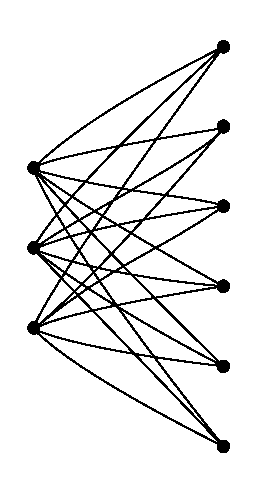
\includegraphics[scale=0.45,page=1]{pictures.pdf}\hspace{2cm}
	    \includegraphics[scale=0.45,page=2]{pictures.pdf}
  \caption{\emph{Left:} Complete bipartite graph $K_{3,6}$. \emph{Right:} The ladder $L_5$.}
  \label{fig:bipartite}
\end{figure}

\begin{example}
	An important role in stability theory is played by what we call \emph{ladder} graphs, defined as follows.
	Fix a number $k\in\N$. The \emph{$k$-ladder} is 
	the bipartite graph denoted $L_k$, with vertex set $V=\set{1,\ldots,k}\times \set{L,R}$ and edge set $E=\setof{\set{(i,L),(j,R)}}{
	1\le i\le j\le k}$. We call the sets $\set{1\ldots,k}\times \set{L}$ and $\set{1,\ldots,k}\times \set R$ the \emph{sides} of the ladder.
  The ladder $L_5$ is depicted to the right in Figure~\ref{fig:bipartite}.	
\end{example}

\begin{example}
  Another family of graphs are the \emph{powerset} graphs,
  defined as follows.
  Let $k\in\N$ be a number, and let $X=\set{1,\ldots,n}$.
  The \emph{$k$-powerset graph} is the bipartite graph denoted $P_k$, with parts $X$ and $P(X)$, 
  and edge set $E=\setof{\set{x,Y}}{x\in X,\ Y\in P(X),\ x\in Y}$. In other words, for every subset $Y$ of part $X$ of the graph there is precisely one vertex of the part $P(X)$
  which is connected to all vertices in $Y$ and to no vertices in $X-Y$.
\end{example}



Let $v,w\in V(G)$.
A \emph{walk} in $G$ is a sequence of vertices $v_0,v_1,\ldots,v_n$
such that  $v_iv_{i+1}$ is an edge in $G$ for $i=0..n-1$. This is a walk
from  $v$ to $w$ (or between $v$ and $w$) if $v=v_0$ and $v_n=v$, and has length $n$.
A \emph{path} is a walk with no repeating vertices.
The \emph{distance} between $v$ to $w$, denoted $\dist(v,w)$, is the length of a shortest walk from $v$ to $w$ (and $\infty$ if there are none). By $N_r^G(v)$ we denote the 
$r$-\emph{neighborhood} of $v$ in $G$, i.e., the
set of vertices of $G$ 
whose distance from $v$ is at most $r$. Often we will omit $G$ in the superscript when it will be understood from the context.
A graph $G$ is \emph{connected} if for every pair of its vertices, there is a walk between them.
The \emph{radius} of a graph $G$ is the smallest number $d\in\N$ such that there is a vertex $x$ with $N^G_d(x)=V(G)$.
 
A graph $G$ is \emph{planar} if, intuitively, it can be depicted on the plane $\R^2$ so that its edges do not intersect, except for perhaps 
at their endpoints\footnote{\label{ft:planar}A formal definition of planarity would require the existence a 
function $f$ (called a planar embedding of $G$) mapping each vertex  $v$ of $G$ to a points $f(v)\in\R^2$, and each 
edge $vw$ of $G$
to a continuous curve  $f(vw)\subset\R^2$ joining $f(v)$ with $f(w)$, so 
that two curves $f(e_1),f(e_2)$ associated to distinct 
edges $e_1,e_2$ intersect only perhaps at the endpoints. Here, by \emph{curve} $\Gamma$ we mean
 the image  of a continuous 1-1 function $\gamma:[0,1]\to\R^2$,
 and by the endpoints of $\Gamma$ we mean $\gamma(0)$ and $\gamma(1)$.
 One can prove that requiring the function to be 
 differentiable, or piecewise-linear, or even linear, would not affect the definition of a planar graph.}.


\paragraph{Representing graphs and algorithms}
We will use two standard data structures for representing graphs,
namely the \emph{adjacency matrix} representation and \emph{adjacency list} representation. Both representations assume an implicit linear ordering of the given graph.
We note that one can be computed from the other in polynomial time, and that the size of each representation is polynomial in terms of the number of vertices of the graph.
We will therefore take the liberty to say that an algorithm 
takes as input a graph $G$ and runs in time polynomial in $G$,
meaning that it takes as input either of the two representations of $G$
and runs in time polynomial in $|V(G)|$. 


%
%
%
%  In both representations, we assume an implicit linear ordering of the vertices of a given graph.
%  Let $G$ be a graph with $|V(G)|=n$ and $V=\set{v_1,\ldots,v_n}$.
%  Let $\#,\$\not\in\set{0,1}$ be two separator symbols.
%  The \emph{adjacency matrix} representation of  $G$
%  consists of the string $\text{bin}(n)\# w$, where
%  $\text{bin}(n)\in\set{0,1}^*$ is the binary representation
%  of $n=|V(G)|$, and $w\in\set{0,1}^*$ is the word of length $n^2$ whose  $m$th bit (where $m\in\set{0,\ldots,n^2-1}$) is set to $1$ precisely if $v_iv_j\in E(G)$, where $i,j\in\set{0,\ldots,n-1}$ are such that $m=i\cdot n+j$.
%
% The \emph{adjacency list} representation of the graph $G$
% consists of the word $\text{bin}(n)\#w_1,\#, w_2 \#,\ldots \# w_n,$
% where $w_i$ is the concatenation of all
 



% Sometimes, when we will want to underline the fact that something is a digraph rather than a graph, we will denote it by $\di G$. Many definitions below
% apply to both graphs and digraphs, so $G=(V,E)$ might denote them.

% Fix a set $C$ of \emph{colors}.
% A \emph{colored graph} (colored by $C$)
% is a graph $G$ together with a function $\col:V(G)\to C$, assigning a color $\col(v)$ to each vertex  $v\in V(G)$.

\paragraph{Subgraphs, embeddings, isomorphisms}
If $G$ is a graph, then a \emph{subgraph} of $G$
is a graph $H$ such that $V(H)\subset V(G)$
and $E(H)\subset E(G)$. We say that $H$
is an \emph{induced} subgraph of $G$
if $E(H)=E(G)\cap (V(H)\times V(H))$.
The subgraph of $G$ induced by a set vertices $W\subset V(G)$ is the graph denoted $G[W]$ with vertices $W$ and edge set $E(G)\cap (W\times W)$. 

If $H$ and $G$ are graphs, then an \emph{embedding}
of $H$ into $G$ is a 1-1 function $f:V(H)\to V(G)$
such that for every pair $v,w\in V$, 
$vw$ is an edge of $H$ if and only if $f(v)f(w)$ is an edge of $G$. 
We write $f:H\to G$ when $f$ is an embedding of $H$ into $G$.
We say that $H$ \emph{embeds} into $G$ if there is an embedding of $H$ into $G$.
An \emph{isomorphism} is a surjective embedding.  Note that $H$ embeds into $G$ if and only if $H$ is isomorphic to an induced subgraph of~$G$.


\paragraph{Minors}
Let $G$ and $H$ be two graphs.
% Fix a number $d\in\N$.
A \emph{minor model} of $H$ in $G$
is a mapping $B$
which maps each vertex $v$ of $H$ to a connected subgraph $B(v)$ of $G$,
called the \emph{bag} of $v$,
and each edge $vw$ of $H$ to an edge $B(vw)$ of $G$,
subject to the following conditions
(cf. Figure~\ref{fig:minor}):
 % such that for all $v,w\in V(G)$ the following conditions hold:
\begin{itemize}
	\item Bags of distinct vertices are pairwise disjoint, i.e.,  $V(B(v))\cap V(B(w))=\emptyset$ for all
	 $v,w\in V(H)$ such that $v\neq w$;
	\item For every edge $vw\in E(H)$, the edge $B(vw)$ joins a vertex in $V(B(v))$ with a vertex in $V(B(w))$.
\end{itemize}



\begin{figure}[h]
  \centering
    \includegraphics[scale=0.35,page=6]{pictures.pdf}
  \caption{The graph $H$ depicted above is a minor (at depth $1$) of the graph $G$. The minor model maps a vertex $v$ of $H$ to the subgraph $B(v)$ of $G$ induced by the spot of the same color as $v$,
  and maps an edge $vw$ to the thick edge joining $B(v)$ with $B(w)$.
  }
   \label{fig:minor}
\end{figure}

We say that $H$ is a \emph{minor} of $G$
if there is a minor model of $H$ in $G$. 
The \emph{radius} of a minor 
model is the maximal radius of all of its bags.
If $d\in\N$,
we say that $H$ is a minor of $G$
at \emph{depth} $d$ if there is a minor model of $H$
in $G$ of radius $d$.

\paragraph{Conventions}
Often, the 
behavior of the function
 $B$ on edges will be irrelevant, and it will only matter that 
 for every edge $vw\in E(H)$ there is some edge joining a vertex in $V(B(v))$ with a vertex $V(B(w))$. In this case, the model $B$ can be 
 described by providing its behavior on vertices (i.e, the bags associated to each vertex), and the extension to edges can be chosen arbitrarily. Also, since adding or removing edges to a bag $B(v)$ cannot 
 spoil the model $B$ as long as the bag remains connected, in many cases, we may simply provide the vertex set $W\subset V(G)$ of the bag of $v$, and assume that $B(v)=G[W]$ is the subgraph of $G$ induced by $W$.
 On the other extreme,  
 we may always modify a minor model (without altering its radius) so that each bag is a spanning tree; in this case, we will say that $B$ is a minor model whose bags are trees. 
 


\paragraph{Topological minors}
A \emph{topological minor model} of $H$ in $G$
is a mapping $M$ 
mapping vertices of $H$ to vertices of $G$ 
and  edges of $H$ to paths in $G$,
subject to the following conditions:
\begin{itemize}
	\item For every edge $vw\in E(H)$, 
	$M(vw)$ is a path from $M(v)$ to $M(w)$ in $G$,
	\item For every pair of edges $e,f\in E(H)$,
	the paths $M(e)$ and $M(f)$ have no common vertices,
	except for perhaps their endpoints.	
\end{itemize}
Since the behavior of $M$ on vertices can be deduced from the behavior on edges, we will often describe $M$ by simply providing the latter.

We say that $H$ is a \emph{topological minor} of $G$
if there is a topological minor model of $H$ in $G$.
If $d\in \N$, we say that $H$ is a topological minor of $G$ at \emph{depth} $d$ if there is a topological minor model $M$ of $H$ in $G$ with the property that 
$M(vw)$ is a path of length at most $d+1$, for each edge $vw\in E(H)$.


\begin{figure}[h]
  \centering
    \includegraphics[scale=0.35,page=7]{pictures.pdf}
  \caption{The graph $H$ depicted above is a topological minor (at depth $2$) of the graph $G$. The minor model maps a vertex $v$ of $H$ to the vertex of $G$ with the same color, and edges of $H$ to the   paths in $G$ delineated using thick edges.} 
  % \label{fig:bipartite}
\end{figure}

\begin{example}
	Let $G_{k\times k}$ denote the $k\times k$ grid, depicted  in 
	Figure~\ref{fig:grid} to the left, in the case $k=5$. Then every planar 
	graph 
	is a minor of $G_{k\times k}$, for sufficiently large $k$.
	This is illustrated in Figure~\ref{fig:grid}, to the right.
	However, the star with five arms, which is clearly planar, is not a topological minor of any grid $G_{k\times k}$, since it has a vertex of degree $5$, while $G_{k\times k}$ has  vertices of degree at most $4$,
	and topological minors cannot increase the maximal degree.
	
	
	\begin{figure}[h]
	  \centering
	    \includegraphics[scale=0.35,page=5]{pictures.pdf}\hspace{3cm}
	    \includegraphics[scale=0.35,page=9]{pictures.pdf}		
	  \caption{\emph{Left:} The $5\times 5$ grid.
	  \emph{Right:} The planar graph $H$ is a minor of the grid $G_{k\times k}$,
	  for some large $k$.
	  } 
	  \label{fig:grid}
	\end{figure}	

\end{example}

\begin{example}\label{ex:topminor-minor}
	If $H$ is a topological minor of $G$ then $H$ is also a minor of $G$.
	More precisely, if $H$ is a topological minor of $G$ at depth $d$,
	then $H$ is a minor of $G$ at depth $\lceil d/2 \rceil$.
	Indeed -- a topological minor model $M$ of $H$ in $G$
	can be converted into a minor model $B$ of $H$ in $G$, as follows.
	For each edge $vw\in E(H)$, consider the path $M(vw)$ joining $M(v)$
	with $M(w)$. Distribute the vertices along this path, by assigning a vertex $w\in M(vw)$ 
	to either $B(v)$ or $B(w)$, depending on whether its is closer to $M(v)$
	or to $M(w)$ along the path (in case of a tie, choose arbitrarily).
	Note that the vertices added to $B(v)$ have distance at most $\lceil d/2\rceil$ to $M(v)$.
	By repeating this for each edge $e$ in $E(H)$, we have constructed a set $B(v)$, for each $v\in V(H)$. We identify this set with the subgraph of $G$ which it induces. Then $B$ is a graph minor model of $H$ in $G$.
\end{example}

\begin{lemma}\label{lem:minor-transitivity}
  If $G_1\in\minors {d_1} {G_2}$ and $G_2\in\minors {d_2} {G_3}$,
  then $G_1\in\minors d {G_3}$, where $d=\ldots$.
  Similarly, 
  if $G_1\in\tminors {d_1} {G_2}$ and $G_2\in\tminors {d_2} {G_3}$,
  then $G_1\in\tminors d {G_3}$, where $d=\ldots$.
\end{lemma}



\paragraph{Subdivisions}
If $G=(V,E)$ is a graph and $e$ is its edge,
then \emph{subdividing} this edge  $k$ times results in replacing the edge $e$
by a path of length $k+1$, as depicted to the left in Figure~\ref{fig:subdivision} in the case $k=2$.


\begin{figure}[h]
  \centering
    \includegraphics[scale=0.35,page=3]{pictures.pdf}\hspace{2cm}    \includegraphics[scale=0.35,page=4]{pictures.pdf}
  \caption{\emph{Left:} The process of subdividing an edge two times.
  \emph{Right:} The maximal 1-subdivision of $K_5$.
  } 
  \label{fig:subdivision}
\end{figure}


A $k$-\emph{subdivision} of the graph $G$
is any graph obtained by subdividing each of its edges
at most $k$ times. The vertices of the original graph $G$
are called the \emph{principal} vertices of the resulting subdivided graph.
The \emph{maximal} $k$-subdivision of $G$ is obtained by subdividing each edge of $G$ exactly $k$ times. The maximal $1$-subdivision of $K_5$
is depicted in  Figure~\ref{fig:subdivision}, to the right.




The following lemma relates subdivisions to topological minors.
\begin{lemma}\label{lem:minors-subdivisions}
  Let $H,G$  be graphs. Then
  	$H$ is a topological minor of $G$ at depth $d$
  	if and only if some $d$-subdivision of $H$
  	is isomorphic to a subgraph of $G$.
\end{lemma}


\paragraph{Graph congruences}
Let $G$ be a graph and let $\sim$ be an equivalence relation on $V(G)$. Then $\sim$ is a \emph{congruence} of $G$ if 
whenever $v_1,w_1,v_2,w_2\in V(G)$ are such that 
 $v_1\sim v_2$ and $w_1\sim w_2$, then $v_1w_1\in E(G)$ if and only if $v_2w_2\in E(G)$. In other words,
  for any two equivalence classes $c,d\in V(G)/{\sim}$, the graph $G[c\cup d]$ is either a complete bipartite graph with parts $c,d$, or has no edges. In particular, taking  $c=d$, we see that $G[c]$ has no edges for each equivalence class $c$.
 We denote by $G/{\sim}$ the quotient graph,
 with vertex set $V(G)/{\sim}$, in which two equivalence classes $c,d\in V(G)/{\sim}$ are adjacent precisely when $G[c\cup d]$ is the complete bipartite graph with parts $c,d$. Observe that the quotient graph $G/{\sim}$ is isomorphic to an induced subgraph of $G$: if  $f:V(G/{\sim})\to V(G)$ is any mapping which maps an equivalence class $c\in V(G)$ to any of its elements, then $f$ is an embedding of $G/\sim$ into $G$.
 
 

\section{Preliminaries on logic}
In this section, we recall some basic definitions from logic. We start from defining relations, which we call here {tables} for brevity.



\paragraph{Tuples and tables}
Let $X$ and $Y$ be two sets.
We will sometimes call a function from $X$ to $Y$
a \emph{tuple over $X$}, or \emph{indexed by} $X$, with \emph{values from} $Y$. 
If we omit the set $Y$ from this notation, and 
just talk about a tuple over $X$, then~$Y$ is allowed to be an arbitrary set. 
If $t$ is a tuple over $X$ and $U\subset X$, then
by $t[U]$ we denote the tuple obtained from restricting the tuple $t$ to $U$. For $x\in X$ we will also write $t[x]$ to denote $t(x)$, and call $t[x]$ the \emph{value} of $t$ at \emph{position} $x$.
We also say that $t[x]$ is an \emph{element} of the tuple $t$.
For defining tuples, we may use the $\mapsto$ notation, e.g., $\set{x\mapsto 1,y\mapsto 2}$
denotes the tuple $t$ such that $t[x]=1$ and $t[y]=2$.
If $n\in\N$, then an \emph{$n$-tuple} $t$ is a tuple over $\set{1,\ldots,n}$. The tuple $\set{1\mapsto y_1,\ldots,n\mapsto y_n}$ can be also denoted $(y_1,\ldots,y_n)$. We may also simply that $y_1,\ldots,y_n$ is a tuple of elements.
The \emph{empty tuple}, denoted $\eps$, is the unique tuple $\eps:\emptyset\to\emptyset$ indexed by $\emptyset$.



If $t$ is a tuple over $X$ with values from $Y$,
and $f:Y\to Y'$ is a function, then by $f(t)$
we denote the tuple over $X$ with values from $Y'$ obtained by applying $f$ element-wise, i.e., $f(t)[x]=f(t[x])$ for $x\in X$.

A \emph{table over} $X$ (with values from $Y$) is a set of tuples over $X$ (with values from $Y$).
If $T$ is such a table and $U\subset X$, then by 
$T[U]$ we denote the set of all tuples $t[U]$, for $t\in T$.
There are two tables over $\emptyset$: the empty table, and the table consisting of the empty tuple $\eps$.

% If $Y$ is a set, then  $\Fun X Y$ denotes the table consisting of all tuples over $X$ with values from $Y$.





\paragraph{First-order logic}
Fix an infinite, countable set of \emph{variables} $\Vv=\set{x,y,\ldots}$.
We inductively define the syntax  of \emph{formulas} for graphs.
Every formula $\phi$ will additionally have an associated set of \emph{free variables}
$\fv(\phi)\subset \Vv$.

\begin{itemize}
	\item $\top$ and $\bot$ are formulas with no free variables.
	\item If $x,y$ are variables then $x=y$ and $xy\in E$ are formulas. For each of them, the set of free variables is $\set{x,y}$.
	\item If $\phi,\psi$ are formulas, then $\phi\land \psi,\phi\lor\psi,\phi\implies\psi,\phi\iff\psi$ are formulas with free variables $\fv(\phi)\cup\fv(\psi)$, and $\neg\phi$ is a formula with free variables $\fv(\phi)$.	
	
	\item If $\phi$ is a formula and $x$ is a variable then $\forall x.\phi$ and $\exists x. \phi$ are formulas, whose set of free variables is $\fv(\phi)-\set x$.
\end{itemize}



The semantics of formulas is also defined by induction.
Fix a graph $G=(V,E)$. 
% If $X$ is a set of variables, then a \emph{valuation} of $X$ in $G$ is a function $\val :X\to V$. We also write $\val \in V^X$.
For a formula $\phi$ with free variables $X$ we inductively define its \emph{semantics} in $G$, denoted $\sem \phi_G$, which is a table
over $X$ with values from $V$, i.e., $\sem \phi_G\subset (\Fun X V)$:
\begin{itemize}
	\item If $\phi$ is $\top$, then 
	$\sem \phi_G$ is the table $\set{\eps}$ over $\emptyset$ consisting only of the empty tuple $\eps$.
	
	\item If $\phi$ is $\bot$, then 
	$\sem \phi_G$ is the empty table over $\emptyset$.	
	
	\item If $\phi$ is of the form $x=y$, then
	$\sem \phi_G$ consists of all those tuples $\fun \val {\set {x,y}} V$,
	such that $\val[x]=\val[y].$

	\item If $\phi$ is of the form $xy\in E$, then
	$\sem \phi_G$ consists of all those tuples $\fun \val {\set {x,y}} V$,
	such that $\val[x]\val[y]\in E.$
		
	\item If $\phi$ is of the form $\exists x.\psi$, then
	$\sem \psi_G=\sem \phi_G[\fv(\phi)].$ In other words,
	$\sem\psi_G$ consists of those tuples $s$ over $\fv(\phi)$, which extend to some tuple $t$ over $\fv(\psi)$ such that $t\in \sem \psi_G$.
	
	\item If $\phi$ is of the form $\psi\lor \gamma$, then $\sem \phi_G$
	is defined as the set of those tuples $\fun\val {\fv(\psi)\cup\fv(\phi)} V$,
	such that $\val[{\fv(\phi)}]\in \sem \phi_G$ or $\val[{\fv(\psi)}]\in \sem \psi_G$ (or both).
	
	\item If $\phi$ is of the form $\neg\psi$, then $\sem\phi_G=(\Fun {\fv(\psi)} V) - \sem\psi_G$, i.e., 
	$\sem \phi_G$ consists of all tuples $t$ over $\fv(\psi)=\fv(\phi)$ such that $t$ does not belong to $\sem\psi_G$.
	

\item The semantics for $\forall x.\phi$ is defined as the semantics of $\neg\exists x.\neg\phi$, and the semantics of $\phi\land \psi,\phi\implies\psi,\phi\iff\psi$ is defined as usual using $\lor$ and $\neg$.
\end{itemize}


This finishes the definition of formulas of first-order logic for graphs. In this paper, when we say \emph{formula} we implicitly mean such a formula, unless stated otherwise.
A formula $\phi$ with no free variables is called a \emph{sentence}. The variables which occur in a formula, but are not free are called \emph{bound} variables.
The \emph{size} of a formula is the number of symbols it consists of.
Note that there are finitely many formulas of a fixed size.
Two formulas $\phi, \psi$ with $\fv(\phi)=\fv(\psi)$ are \emph{equivalent} if for any (finite or infinite) graph $G$, $\sem\phi_G=\sem\psi_G$.
Note that $\top$ 
is equivalent to $\forall x.x=x$, $\bot$ is equivalent to $\exists x.\neg (x= x)$,
so the formulas $\bot$ and $\top$, as well as the constructs 
$\land,\implies,\iff,\forall$
 are (up to equivalence) redundant in our definition of first-order logic, and in the inductive proofs it is enough to assume that formulas do not use these constructs, and use only the constructs $x=y, xy\in E$
 (called the \emph{atomic} formulas) and the boolean connectives
 $\lor,\neg$.

\begin{proposition}\label{pro:fo-evaluation}
	Fix a formula $\phi$. For a given graph $G$, 
	the table $\sem\phi_G$ can be computed in time polynomial in $G$.
\end{proposition}
\begin{proof}	
	The proof proceeds by induction on the structure of the formula $\phi$. We  represent tables in the standard way, as arrays.
	The base case consists of the atomic formulas $xy\in E,x=y$, for which the claim holds, assuming either the adjacency matrix or adjacency list representation of the input graph $G$. In the inductive step, when $\phi$ is of one of the forms $\exists x.\psi,\ \psi\lor\gamma$, or $\neg \psi$, we observe that the definition of the semantics gives a naive evaluation algorithm of $\sem\phi_G$ from $\sem\psi_G$ and $\sem \gamma_G$.
\end{proof}


\paragraph{Conventions}
If $\cal F$ is a finite set of formulas, then we may write 
$\bigvee \cal F$ to denote $\phi_{1}\lor \phi_{2}\lor\ldots \phi_{n}$, where $\phi_1,\ldots,\phi_n$ is an enumeration of $\cal F$ in any order. Similarly, 
if $\family{\phi_i}{i\in I}$ is a finite family of formulas, then  $\bigvee_{i\in I} \phi_i$ denotes
$\bigvee \setof{\phi_i}{i\in I}$. This convention applies also to $\bigwedge$ in place of~$\bigvee$.
Also, we will often write $\exists x_1\ldots x_n.\phi$ as  shorthand for $\exists x_1.\exists x_2\ldots\exists x_n.\phi$.
We use $x\neq y$ as shorthand for $\neg (x=y)$.

When $\val\in\sem \phi_G$, we may also say that $\val$ \emph{satisfies}
the formula $\phi$ in~$G$. We may also skip the graph $G$,
if it is understood from the context.
 If $\phi$ is a formula with 
free variables $X$, and an assignment $t$ of some vertices
$v_1,\ldots,v_n\in V(G)$  to $X$ is implicit,
then we may say that $v_1,\ldots,v_n$ 
satisfies the formula $\phi$, whenever  $t$ satisfies $\phi$ in $G$. In particular, if $X=\set x$ is a singleton, 
then we will often say that $v\in V(G)$ satisfies $\phi$,
meaning that  $t\in \sem \phi_G$, where $t:X\to V(G)$ is  such that $t[x]=v$. In the extreme case when
$\phi$ is a sentence and $X=\fv(\phi)=\emptyset$, then $\sem \phi_G$
is a subset of $\set\varepsilon$, where $\varepsilon$
is the {empty tuple}. In particular, $\sem\phi_G$ is either empty  or $\sem\phi_G=\set\varepsilon$. In the latter case we say that $\phi$ is satisfied in $G$, or $\phi$ holds in $G$. 

Any formula $\phi$ with free variables $X$ can be treated as a formula with free variables $Y$, for a set $Y$ containing $X$: it is enough to replace $\phi$
by the formula $\phi\land \bigwedge_{y\in Y}(y=y)$.
Therefore, in the sequel, when saying $\phi$
\emph{is a formula with free variables} $Y$, we will actually also allow $\phi$ to be a formula with $\fv(\phi)\subset Y$. 
We may write $\phi(x,\ldots,z)$ 
to indicate that $\phi$ is treated as a formula with free variables $x,\ldots,z$. For instance, we may write
$\phi(x,y)=\top$, which means that $\phi$ is the formula with free variables $x,y$, obtained from $\top$ as described above,
i.e., $\phi=\top\land(x=x)\land (y=y)$.

If $\phi$ is a formula and $s:\fv(\phi)\to\Vv$ is a function, then by $\phi\, s$ we denote the formula 
$\psi$ obtained by substituting the free variables of $\phi$
according to $s$. For example, 
If $\phi$ is the formula $xy\in E$ then $\phi\, \set{x\mapsto p,y\mapsto r}$ is the formula $pr\in E$.
One has to be careful when substituting the free variables:
 first rename all bound variables in $\phi$
by fresh variables (i.e., not appearing in $\phi$ nor in~$s$), and then rename the free variables according to $s$. For example, if $\phi$ is the formula $\exists y.xy\in E$ then $\phi\,\set{x\mapsto y}$ is the formula $\exists z.yz\in E$, where $z$ is some fresh variable.


Finally, whenever $\textit{desc}$ is any mathematical description of a property
(using words, formulas, or their combination) of some elements $x,\ldots,z$ which is known to be definable by some  first-order formula $\phi(x,\ldots,z)$, then by $[desc]$ we mean the formula $\phi$.
For instance, we will show in Example~\ref{ex:dist} 
that for any fixed $d\in \N$ there is a first-order formula $\phi(x,y)$ expressing the property 
``$x$ and $y$ are at distance at most $d$'', i.e., $\dist(x,y)\le d$. Then $[\dist(x,y)\le d]$ is shorthand for the formula $\phi$.




\begin{example}\label{ex:walk}
	Let $\phi$ be the formula $$\exists x_0.\exists x_1.\exists x_2.\exists x_3.(x=x_0)\land (x_0x_1\in E)\land (x_1x_2\in E)\land (x_2x_3\in E)\land (x_3=y),$$
	which can be also written as $\exists x_0\ldots x_3. (x=x_0)\land (x_3=y)\land\bigwedge_{i=0..2} (x_ix_{i+1}\in E)$. Then $\fv(\phi)=\set{x,y}$.
	For a graph $G=(V,E)$, the set $\sem \phi_G$ consists of all tuples
	$\set{x\mapsto v,y\mapsto w}$ such that $v,w\in V$ and there is a walk from $v$ to $w$
	of length exactly $3$. For each such a tuple, we may also say that the pair of vertices $v,w\in V(G)$ satisfies $\phi$.
\end{example}
	
\begin{example}\label{ex:dist}
	In a similar way, we may write a first-order formula 
	$\phi^d$ expressing the property that $\dist(x,y)\le d$, for a fixed value $d\in\N$:
	$$\phi^d\ =\bigvee_{d=0..r}\left(\exists x_0\ldots x_r. (x=x_0)\land (x_r=y)\land\bigwedge_{i=0..d} (x_ix_{i+1}\in E)\right).$$ 
\end{example}	

\begin{example}\label{ex:deg}
	For a fixed $k\in\N$, the  formula $$\delta_{\ge k}\ =\ \exists x_1\ldots x_k \bigwedge_{1\le i<j\le k} \neg(x_i=x_j)\land \bigwedge_{1\le i\le k}
	(x_ix\in E)$$ with free variable $x$ expresses the property that $x$ has degree at least $k$.
	The formula $\delta_{\ge k}\land \neg\delta_{\ge {k+1}}$ expresses the property that $x$ has degree exactly $k$.
\end{example}



\begin{example}
  The following sentence $\psi$ expresses the property that
  a graph has an \emph{independent set of size $k$}:
  $$\psi=\exists x_1\ldots x_k.\bigwedge_{1\le i<j\le k}\neg[\dist(x_i,x_j)\le 1].$$
  More explicitly,
$$\psi=\exists x_1\ldots x_k.\bigwedge_{1\le i<j\le k}\neg((x_i=x_j)\lor (x_ix_j\in E)).$$

	The following sentence $\phi$ expresses the property that a graph has \emph{a dominating set of size $k$}:
  $$\phi=\exists x_1\ldots x_k.\forall x.\bigvee_{i=1..k}[\dist(x,x_i)\le 1].$$
  More explicitly,
  $$\phi=\exists x_1\ldots x_k.\forall x.\bigvee_{i=1..k}
  (x=x_i)\lor (xx_i\in E).$$
\end{example}

\begin{example}\label{ex:ladder}
  This example shows that using a fixed formula $\phi(x,y)$, one can define a partial order $\leqslant$
  on the vertices of the ladder $L_k$, 
  so that for two vertices $v,w\in V(L_k)$,
  $v\leqslant w$ if and only if $v$ and $w$
  are on the same side of the ladder, and $\deg(v)\le \deg(w)$ (see Figure~\ref{fig:ladder-order}).
  \begin{figure}[h]
    \centering
      \includegraphics[scale=0.35,page=14]{pictures}
    \caption{The ordering of the ladder.}
    \label{fig:ladder-order}
  \end{figure}
    Note that the degrees of the vertices on one side of the ladder are $1,2,\ldots,k$; in particular, they are unbounded, for unbounded $k\in\N$, so it is not immediately clear how to order the vertices according to the degree using a fixed formula. However, observe that 
    in the ladder $L_k$,
    if $x,y$ are two vertices on the same side of the ladder,
    then $\deg(x)\le \deg(y)$ if and only if $N_1(x)\subset N_2(y)$. The property $N_1(x)\subset N_2(y)$ is defined by the following formula:
  \begin{align*}
    \phi(x,y)&=\forall z.(xz\in E)\implies (yz\in E).
  \end{align*}
Hence, $\phi(x,y)$ if and only if $x\leqslant y$.

We now define a formula $\psi(x,y)$ which defines a bijection between the two sides of the ladder $L_k$,
which matches every vertex on one side with the corresponding vertex on the other side. The formula $\psi(x,y)$
expresses the property: $y$ is the smallest neighbor of $x$,
with respect to the linear order defined by $\phi$:
\begin{align*}
  \psi(x,y)&=(xy\in E)\land \forall z.\big((xz\in E)\implies(\phi\,\set{x\mapsto y,y\mapsto z})\big).
\end{align*}
\end{example}



\paragraph{Locality}
In this section, we recall the notion of Gaifman locality for first-order logic. 
Fix a graph $G$ and a number $d\in\N$. Let $t$ be a tuple over a set $X$, consisting of vertices of $G$.
By $N_d(t)$ we denote the subgraph of $G$ induced by the set of vertices of distance at most $d$ from some element of the tuple $t$.
If $t,s$ are two such tuples, we say that they have \emph{isomorphic} 
$d$-neighborhoods if there is an isomorphism  $f:N_d(t)\to N_d(s)$
which maps $t$ to $s$, i.e., $f(t)=s$. 
A $d$-\emph{neighborhood type} over $X$ is an equivalence class
of the relation of having isomorphic $d$-neighborhoods. 
A $d$-neighborhood type over $X$ can be represented by a graph $T$, together
with a distinguished tuple of vertices $t$ indexed by $X$, i.e.,
$t:X\to V(T)$, with the property that $N_d(t)=T$.
\sz{pic of $d$-neighborhood type}

We say that a formula $\phi$ is \emph{$d$-local} if for every graph $G$
and for every two tuples $s,t$ over $\fv(\phi)$ with isomorphic $d$-neighborhoods, 
either both $s,t$ belong to $\sem\phi_G$, or both $s,t$ do not belong to $\sem\phi_G$. In other words, whether a tuple $t$ of vertices of $G$ satisfies $\phi$ depends only on the $d$-neighborhood type of  the tuple $t$ (as well as of global properties of $G$, independent on the choice of the tuple $t$).

\begin{theorem}[Gaifman's locality]\label{thm:gaifman}
	Let $\phi$ be a formula of first-order logic for graphs.
	Then there is a number $d\in\N$ such that $\phi$ is $d$-local.	
	Moreover, the number $d$ can be computed from $\phi$.
\end{theorem}

\sz{Perhaps the theorem about Gaifman normal form would be more useful}
\begin{example}
	For $n\in\N$, let $P_n$ denote the graph with vertices $v_0,\ldots,v_n$ whose edges are pairs $v_{i}v_{i-1}$, for $i=1,\ldots,{n}$. 
	The graph $P_n$ is called the \emph{path} of length $n$; the vertices $v_0$ and $v_n$ are called the endpoints. There is a formula $\phi(x)$ such that a vertex $v\in V(P_n)$ satisfies $\phi$ if and only if $v$ is an endpoint -- indeed, it suffices to take the formula $\neg\delta_{\ge 2}$ from Example~\ref{ex:deg}. There is no formula $\psi(x)$
	such that $v\in V(P_n)$ satisfies $\psi$ if and only if $v=v_0$. Intuitively, the vertices $v_0$ and $v_n$
	of $P_n$ are indistinguishable by first-order logic. One does not even need Gaifman locality to prove this -- it is sufficient to
	 observe (and prove by induction)  that the semantics of first-order logic is preserved under isomorphism, i.e., if $s$
	and $t$ are two tuples of elements of $G$ and there is an isomorphism $f:G\to G$ which maps $s$ to $t$, then $s\in \sem\phi_G$
	if and only if $t\in \sem \phi_G$. Clearly, there is an isomorphism of $P_n$ to $P_n$ which maps $v_0$ to $v_n$.
	
		
	
	
	For each \emph{fixed} $n$  there is a formula $\textit{even}_n(x)$ such that $v\in V(P_n)$ satisfies $\textit{even}_n(x)$ if and only there is an even-length path from $v$ to one of the endpoints of $P_n$ -- it suffices to take $$\textit{even}_n(x)=	
	\bigvee_{k=0..n}
	(\exists y.
	[\deg(y)=1]\land
	[\dist(x,y)=2k]).$$
	However, the size of any  formula expressing this property necessarily depends on $n$.
	Indeed, suppose that  $\phi$ is a formula with one free variable $x$.
	% such that for all numbers $m,n\in N$ such that $m\le 2n$,
	%  $v_m$ satisfies $\phi$ in $P_{2n}$ if and only if $m$ is even.
	 Let $d$ be the number from Gaifman's locality theorem. 
	 Then for any $k,l,n\in \N$ such that $d< k,l< n-d$,
	 the $d$-neighborhoods of $v_k$ and of $v_l$
	 are isomorphic in $G$, so	 
	 whenever $v_k$ satisfies $\phi$, 
	 also $v_l$ satisfies $\phi$.
\end{example}


% \paragraph{First-order logic for digraphs, colored graphs, colored digraphs}
% The above definition of first-order logic can be applied verbatim to
% digraphs. We can also define first-order logic for colored (di)graphs.
% The definitions of syntax and semantics extend the above definitions, by
% allowing a new formula $\col(x)=c$ for
% each fixed color $c\in C$ and variable $x\in \Vv$. Its set of free variables
% is $\set x$ only (without $c$, since $c$ is fixed).
% Furthermore, for a fixed colored (di)graph $G$ (with an implicit coloring $\col:V(G)\to C$)
% we define the semantics $\sem \phi_G$ of such a formula $\phi$ as the set of those tuples $\val:\set x\to V$ which map $x$
% to a vertex of color $c$ in $V$, i.e., $\col(\val(x))$.

\paragraph{Interpretations}
We now describe how formulas can define new graphs out of old ones. Roughly, the idea is that the vertices of the new graph are tuples of vertices of the old graph 
of a fixed length $d$,
and the edges of the new graph are specified by a formula with $2d$ free variables.

We will use the following notation.
For two sets $X,Y$, denote by $X\disjoint Y$
the disjoint union of $X$ and~$Y$, formally defined as $X\disjoint Y=(X\times\set{1})\cup (Y\times \set {2})$.
For an element $x\in X$, denote $x_1\eqdef (x,1)$ and for an element $y\in Y$, denote $y_2\eqdef(y,2)$.
 If $s$ is a tuple over $X$ and $t$ is a tuple over $Y$, then  $s\disjoint t$ denotes
the tuple over $X\disjoint Y$ defined in the obvious way, so that $(s\disjoint t)[x_1]=s[x]$
and $(s\disjoint t)[y_2]=t[y]$.


An \emph{interpretation} is a pair $\Phi=(\phi_V,\phi_E)$ consisting of two formulas,
$\phi_V,\phi_E$ such that if $\fv(\phi_V)=X$, then
$\fv(\phi_E)=X\disjoint X=\setof{x_1}{x\in X}\cup \setof{x_2}{x\in X}$, the disjoint union of two copies of $X$.
For a given graph $G$, define a new graph $\Phi(G)$ as follows:
\begin{align*}
V(\Phi(G))&\eqdef\sem {\phi_V}_G,&
E(\Phi(G))&\eqdef\setof{\set{s, t}}{s,t\in\sem{\phi_V}_G,\ s\neq t,\ s\disjoint t\in \sem{\phi_E}_G}.
\end{align*}
 If a graph $H$ is isomorphic to a graph $\Phi(G)$,
for some interpretation~$\Phi$, then we say that $H$ \emph{interprets} in $G$.
The \emph{dimension} of the interpretation $\Phi$
is the number of free variables of the formula $\phi_V$, i.e., $|\fv(\phi_V)|$. Note that $\Phi(G)$ has at most $|V(G)|^d$ vertices, if $\Phi$ is an interpretation of dimension $d$.

\begin{remark}
  Observe that in the interpretation $\Phi$,
  the formula $\phi_E$ might be not symmetric,
  i.e., it may be the case that $s\disjoint t\in\sem{\phi_E}_G$ while $t\disjoint s\notin\sem{\phi_E}_G$,
  or may contain self-loops, i.e., it may be the case that $s\disjoint s\in\sem{\phi_E}_G$. Nevertheless, according to the above definition, the resulting graph $\Phi(G)$ contains no self-loops and is undirected.
  It is not difficult to show that any interpretation $\Phi=(\phi_V,\phi_E)$ can be converted into an interpretation $\Phi'=(\phi_V',\phi_E')$ of the same dimension, which is equivalent to $\Phi$, i.e., 
  $\Phi(G)=\Phi'(G)$ for every graph $G$, and moreover such that $\Phi'$ is symmetric and without self-loops.  
\end{remark}




\begin{example}
	Let $\Phi=(\phi_V,\phi_E)$
	be the interpretation in which
	$\phi_V(x,y,z)=\top$, where $\fv(\phi_V)=\set{x,y,z}=:X$, and  $\phi_E$
	is the formula with free variables $X\disjoint X$
	given by:
 $$\phi_E(x_1,y_1,z_1,x_2,y_2,z_2)=
	\neg ((x_1= x_2)\land (y_1=y_2)\land(z_1=z_2)).$$
	For a given graph $G$, the graph
	$\Phi(G)$ is the clique on $|V(G)|^3$ vertices.
	More generally, observe that for any fixed interpretation $\Phi$,
	the size of $\Phi(G)$ is polynomial in the size of $G$, and $\Phi(G)$
	can be computed in polynomial time from $G$.
\end{example}

\begin{example}\label{ex:subdivision-undo}
  Fix a number $k\in \N$.
	Let $H$ be the maximal $k$-subdivision of a graph $G$
	without vertices of degree $2$; for example, $G$ may be $d$-regular, for some $d\ge 3$.
	Then $G$ interprets in $H$, via a 1-dimensional interpretation $\Phi=(\phi_V,\phi_E)$, where
	\begin{align*}
		\phi_V(x)&=\neg[\deg(x)=2]\\
		\phi_E(x_1,x_2)&=[\dist(x_1,x_2)=k+1].
	\end{align*}
  
  Now suppose that $H$ is some (not necessarily maximal) $k$-subdivision of a graph $G$ without vertices of degree 2. Then $G$ still interprets in $H$, via the interpretation $\Psi$ defined below.
  First observe that for any fixed $d\in\N$, the property ``the vertices $x,y$ 
  can be connected by a path of length at most $d$, which passes only through vertices of degree $2$''
  can be expressed by a first-order formula $\psi^d(x,y)$,
  similarly as in the formula $\phi^d$:
  it suffices to add to $\phi^d$ the conjuncts $[\deg(x_i)=2]$
  for $i=1,\ldots,r-1$.
  Define $\Psi$ as the interpretation consisting of the formula $\psi_V(x)=\neg[\deg(x)=2]$,
  and the formula $\psi_E$ obtained from $\psi^{k+1}$ by substituting the variables $x$ by $x_1$ and $y$ by $y_1$.  
\end{example}

\begin{example}
	Interpretations can act as ``filters''.
	Let $\phi$ be a sentence. Then there is an interpretation $\Phi$
	such that $\Phi(G)=G$ if $G$ satisfies $\phi$, and $\Phi(G)$
	is the empty graph otherwise. Indeed, it suffices to take
	$\phi_V(x)=\phi$ (where $x$ does not appear in $\phi$)  and $\phi_E(x_1,x_2)=x_1x_2\in E$.
\end{example}


\begin{example}\label{ex:subdivide}
Consider the following interpretation $\Phi=(\phi_V,\phi_E)$, 
where 
	\begin{align*}
		\phi_V(x,y)&=(x=y)\lor (xy\in E)\\
		\phi_E(x_1,y_1,x_2,y_2)&=([x_1=y_1=x_2]\land (x_2y_2\in E))\lor ((x_1y_1\in E)\land(x_1=y_2)\land (x_2=y_1)).
	\end{align*}
The result of applying $\Phi$ to a graph $G$ is depicted in Figure~\ref{fig:int-subdivide}. It is not difficult to see that for every graph $G$, the graph $\Phi(G)$ is the result of subdividing each edge of $G$
twice. 

\begin{figure}[h]
  \centering
	    \includegraphics[scale=0.3,page=10]{pictures.pdf}
  \caption{The two-dimensional interpretation subdividing each edge twice.}
  \label{fig:int-subdivide}
\end{figure}
\end{example}

% \begin{remark}\label{rem:general-interpretations1}
\begin{remark}\label{rem:general-interpretations}
  In a more general definition of interpretations,
  instead of a pair $\Phi=(\phi_V,\phi_E)$
  one allows a more general form  $\Phi'=(\phi_V,\phi_E,\phi_\sim)$, allowing to further quotient the resulting graph $\Phi(G)$ by a congruence defined by $\phi_\sim$. More precisely,
  suppose that $\fv(\phi_V)=X$ and $\fv(\phi_\sim)=\fv(\phi_E)=X\disjoint X$.
Let
 $$\sim\ =\setof{(s,t)}{s,t\in \sem{\phi_V}_G,\ s\disjoint t\in \sem {\phi_\sim}_G}.$$
 Define $\Phi'(G)$
 as the quotient graph $\Phi(G)/{\sim}$ if the relation 
 $\sim$ is a congruence of  $\Phi(G)$, otherwise let $\Phi'(G)$ be the empty graph. 
  We note that all the results in this paper hold also for the more general form of interpretations.   
% \end{remark}
  
Using the more general notion of interpretation mentioned in Remark~\ref{rem:general-interpretations}, one could modify the interpretation $\Phi$ from Example~\ref{ex:subdivide}, obtaining a generalized interpretation $\Phi'$
which further identifies the elements $(a,b)$  and $(b,a)$
in $\Phi(G)$,
by defining $\Phi'=(\phi_V,[|\set{x_1,y_1}\cap\set{x_2,y_2}|=1], [\set{x_1,y_1}=\set{x_2,y_2}])$ with $\phi_V$ as above.
For a graph $G$, the resulting graph $\Phi'(G)$ is the maximal 1-subdivision of $G$.
\end{remark}


The following lemma shows that interpretations can be composed.

\begin{lemma}\label{lem:interpretation-composition}
	Let $\Phi$ and $\Psi$ be two interpretations. Then there is an interpretation $\Gamma$ such that $\Gamma(G)$ is isomorphic to $\Phi(\Psi(G))$, for every graph $G$.	
\end{lemma}

\paragraph{Types}
Let  $\Delta$ be a set of formulas, $G$ a graph, $A\subset V(G)$  and $v\in V(G)$. We define the $\Delta$-\emph{type} of the vertex  $v$ in $G$ over parameters $A$ as the set consisting of those triples $(\phi,t,x)$ such that $\phi$ is a formula from $\Delta$,
 $\val$ is a tuple satisfying $\phi$, and $x$ is a free variable of $\phi$
such that the tuple $\val$
has value $v$ at position $x$,
and values from $A$ at all remaining positions.
More formally,
$$\tp_\Delta(G,A,v)=\setof{(\phi,\val,x)}{\phi\in\Delta,\ \val\in \sem\phi_G,\ x\in\fv(\phi),\ 
\val[x]=v,\ \val[\fv(\phi)-\set x]\subset A}.$$
The set of $\Delta$-types \emph{realized} in $G$ over $A$
is the set $\setof{\tp_\Delta(G,A,v)}{v\in V(G)}$, denoted
$\rtp_\Delta(G,A)$.
% If $\Delta$ is a set of formulas, then by $\tp_\Delta(G,A,v)$
% we denote the family $\family{\tp_\phi(G,A,v)}{\phi\in\Delta}$.

\begin{example}
	Let $\Delta^r$ denote the set consisting of the single formula 
	$\phi^r(x,y)=[\dist(x,y)\le r]$.
	Let $G$ be a graph and let $A\subset V(G)$.

	\begin{enumerate}
		\item For $v\in V(G)$, we can identify $\tp_{\Delta^r}(G,A,v)$ with $N_r^G(v)\cap A$. Indeed, $\sem {\phi^r}_G$ corresponds to the set of pairs of vertices of $G$  whose mutual distance is at most $r$,
		and $\tp_{\Delta^r}(G,A,v)$ consists of those triples $(\phi^r,t,x)$ such
		that $t[x]=v$ and $t[y]\in A$ and $\dist(t[x],t[y])\le r$,
		and triples $(\phi^r,t,y)$ such that $t[y]=v$ and $t[x]\in A$
		and $\dist(t[x],t[y])\le r $.

		\item Let $G$ be the full graph on $k$ vertices.
		Then $|\rtp_{\Delta^1}(G,A)|=1$.
		
		\item Let $G$ be the $k$-ladder $L_k$.
				Then $|\rtp_{\Delta^1}(G,A)|=2k$.
		
		\item If $G$ is an arbitrary graph, then we can have $|\rtp_{\Delta^1}(G,A)|=2^{|A|}$. Indeed, this happens for instance if 
		$G$ is the bipartite graph with one part consisting of elements of $A$
		and the other part consisting of subsets of $A$,
		with an edge joining a subset of $A$ with all its elements. 
		

		
	\end{enumerate}
	
\end{example}
\section{Graph classes}
In this paper, we are mostly interested in classes of finite graphs\footnote{A class is a notion similar to that of a set, but classes can be larger than sets -- i.e., all finite graphs do not form a set, but form a class. For the purpose of this paper, we could identify a class of graphs $\Cc$ with a property $P$ of graphs expressed in mathematical language (such as e.g. planarity), and instead of writing $G\in\Cc$,
we would say that $G$ has  property $P$.
We could also avoid using classes and talk only about sets, but this would require restricting the vertex-sets of the considered graphs to subsets of some fixed set, e.g. $\N$. All the results in this paper would remain valid, but in the proofs we would have to pay a bit more attention to make sure that all constructed graphs only have natural numbers as vertices.}. 
By $\Gr$ we denote the class of all finite graphs,
and by $\Cc\subset \Gr$ we denote a class of finite graphs. Throughout this paper, unless stated otherwise, when speaking of graphs, we assume them to be finite.
Moreover, we  identify two graphs if they are isomorphic. 
In particular, we assume that every graph class $\Cc$ is closed under isomorphism, i.e., if $G,H$ are isomorphic graphs and $G\in\Cc$, then also $H\in \Cc$. 
By $\cliques$ we denote the class of all cliques.

\begin{example}\label{ex:classes}
Below are several classes of graphs which are of interest 
in this paper.
\begin{enumerate}
	\item The class $\cal P$ of all \emph{planar} graphs. A  graph is planar if and only if neither the clique $K_5$ nor the complete bipartite graph $K_{3,3}$ is its minor. Incidentally, planar graphs are exactly those which do not contain $K_5$ nor $K_{3,3}$ as a \emph{topological} minor.

	\item More generally, for any graph $H$, we may consider the class $\Mm_H$ of all graphs $G$ which \emph{exclude $H$ as a minor}, i.e., graphs $G$ such that $H$ is not a minor of $H$. If $H$ is a graph with at least one edge and $\Cc$ is a class of graphs contained in $\Mm_H$, then we say that the class $\Cc$
	\emph{excludes} a minor.
	Similarly we define the class $\Tt_H$ of all graphs $G$ which \emph{exclude $H$ as a topological minor},
	and say that a class $\Cc$ excludes a topological minor if it is contained in $\Tt_H$, for some graph $H$ with at least one edge. Note that every class which excludes a  minor in particular excludes a topological minor.
	
	
	\item The class ${\cal D}_d$ of all graphs in which all vertices have degrees bounded by $d$.
	This class does not exclude any graph $H$ as a minor. Indeed, for any fixed $n$, the clique $K_n$
	is a minor of a $3$-regular graph $G$ obtained by replacing every vertex $i\in\set{1,\ldots,n}$ in $K_n$ by a path $P^i$ of length $n-1$,
and replacing the $n-1$ edges leaving from $i$	in $K_n$ by $n-1$ edges leaving from consecutive vertices of $P^i$. However, ${\cal D}_d$ is a class which excludes a topological minor, e.g., it excludes $K_{d+1}$ as a topological minor.
	
	\item The class of all graphs of treewidth bounded by a fixed number $d$. We omit the definition of treewidth here, see e.g.~\cite{??}. The class of all graphs of treewidth at most $d$ excludes a minor. More precisely, there is a function $f:\N\to\N$ such that 
	every graph of treewidth $d$ excludes the $k\times k$ grid as a minor where $k=f(d)$.


\end{enumerate}
\end{example}
%
% \subsection{Graph parameters}
% A \emph{graph parameter} is a function $f:\Gr\to \Rbar$, where $\Rbar=\R\cup\set{-\infty,+\infty}$, which is invariant under isomorphism, i.e., $f(G)=f(H)$ for isomorphic graphs $G,H$.
% For example, denote by $\omega(G)$ the maximal number of vertices of a clique $H$ contained (as a subgraph) in $G$.
% Then $\omega$ is a graph parameter.
%
% We consider several graph parameters.
% \begin{itemize}
%   \item For $d\in\N$, let $\omega_d(G)$ denote the maximal number $n$ such that $K_n$ is a minor at depth $d$ of $G$.
%
%   \item Similarly, for  $d\in\N$, let $\tilde\omega_d(G)$ denote the maximal number $n$ such that $K_n$ is a topological minor at depth $d$ of $G$.
%
% \item For $d\in\N$, let $\nabla_d(G)$ denote the maximum
% of $\frac{|E(H)|}{|V(H)|}$, ranging over all graphs $H$ such that $H$ is a minor at depth $d$
% of $G$.
%
% \item For $d\in\N$, let $\nabla_d(G)$ denote the maximum
% of $\frac{|E(H)|}{|V(H)|}$, ranging over all graphs $H$ such that $H$ is a topological minor at depth $d$
% of $G$.
% \end{itemize}
%
%
% Theorem~\ref{thm:nowhere-dense} expresses the fact that in some sense, the  the above graph parameters are all equivalent. To make this equivalence precise, we make the following definitions.
%
% A \emph{graph parameter sequence} is a sequence $f_1,f_2,\ldots$ of graph parameters. Such a sequence will be denoted $f\seq$. If $f\seq$ and $g\seq$ are two graph parameter sequences, then we write that $f\seq\preceq g\seq$
% if there exist increasing functions $s,t:\N\to\N$
% such that $f_n(G)\le s(g_{t(n)}(G))x$, for every graph $G$.
% If $f\seq\preceq g\seq$ and $g\seq\preceq g\seq$, then we write $f\seq \simeq g\seq$.
%
% \begin{theorem}\label{thm:nowhere-dense1}
%   The graph parameter sequences $\omega\seq,\tilde\omega\seq,\nabla\seq,\tilde\nabla\seq$
%   are all equivalent with respect to $\simeq$.
% \end{theorem}

\paragraph{Class operations}
We introduce some convenient notation for applying operations to graph classes.
If $\Phi$  is an interpretation and $\Cc$ is a class of finite graphs, then by $\Phi(\Cc)$ we denote the class $\setof{\Phi(G)}{G\in \Cc}$.

Let $R$ be a binary relation on graphs, i.e., a class $R\subset \Gr\times \Gr$.
By $R(\Cc)$ we denote the class of all graphs $H$
such that the relation $R$ holds of $H$ and $G$, for some graph $G\in \Cc$, i.e.,
$$R(\Cc)=\setof{H\in \Gr}{\exists G\in \Cc. (H,G)\in R}.$$
For example, define the relation $\subgraph$
so that $(H,G)\in\subgraph$ if and only if $H$
is isomorphic to a subgraph of $G$. Then $\subgraph(\Cc)$
is the class of all subgraphs of graphs from $\Cc$.
Similarly, $\minor{}(\Cc)$ denotes the class of all graphs which are a minor of a graph in $\Cc$,
$\minor d (\Cc)$ denotes the class of all graphs which are a minor at depth $d$ of some graph $G\in\Cc$,
and $\tminor d (\Cc)$ denotes the class of all graphs which 
are a topological minor at depth $d$ of some graph $G\in 
\Cc$. Incidentally, $\minor 0 (\Cc)=\tminor 0 
(\Cc)=\subgraph(\Cc)$. Consistently with the above 
convention, $\indsub(\Cc)$ denotes the class of all induced 
subgraphs of graphs in $\Cc$.
A class $\Cc$ is \emph{closed under subgraphs} if $\Cc=\subgraph(\Cc)$, is \emph{closed under induced subgraphs} if $\Cc=\indsub(\Cc)$, and is \emph{minor-closed}
if $\Cc=\minor{}(\Cc)$.
By  $\subdiv k\Cc$ (respectively, $\msubdiv k \Cc$) we denote the class of graphs $H$
such that $H$ is the (maximal) $k$-subdivision of some graph in $\Cc$.




\subsection{Nowhere-denseness}
% For a class of graphs $\Cc$ and a number $d$,
% let $\minors d\Cc$ denote the class
% of all graphs which are a minor at depth $d$
% of some graph $G\in\Cc$. Similarly, by $\tminors d \Cc$ we denote the class of all graphs which are a topological minor at depth $d$ of some graph $G\in\Cc$.
%

The main result presented in this section is the following theorem.
\begin{theorem}\label{thm:nowhere-dense}
	Let $\Cc$ be a class of graphs. 
	The following conditions are equivalent.
	\begin{enumerate}
		\item\label{it:clique-minor}  $\minors d\Cc=\Gr$ for some $d\in\N$.
		In other words, 
		there is a number $d\in\N$ such that 
		every graph $H$ is a minor at depth $d$ 
		of some graph $G\in\Cc$.
		
		\item\label{it:clique-topminor}  $\tminors d\Cc=\Gr$ for some $d\in\N$. %In other words, there is a number $d\in\N$ such that 
%		every graph $H$ is a topological minor at depth $d$ 
%		of some graph $G\in\Cc$.
		
		\item\label{it:dense-minor} There is a number $d\in \N$ and a number 
		   $\eps>0$ such that 
		there are arbitrarily large graphs $H\in\minors d\Cc$ with $\frac{|E(H)|}{|V(H)|}> |V(H)|^{1-\eps}$.
		
		\item\label{it:dense-topminor} There is a number $d\in \N$ and a number 
		   $\eps>0$ such that 
		there are arbitrarily large graphs $H\in\tminors d\Cc$ with $\frac{|E(H)|}{|V(H)|}> |V(H)|^{1-\eps}$.
	\end{enumerate}
\end{theorem}


We say that a class $\Cc$ is \emph{somewhere dense}
if it satisfies one of the equivalent conditions above;
otherwise it is called \emph{nowhere dense}.
In particular, $\Cc$ is nowhere dense if and only if it satisfies one of the following, equivalent conditions.

\begin{align}
  \label{char:nd}\tag{ND1}
\begin{minipage}[c]{0.8\textwidth}\it\noindent For every $d\in \N$ there is a graph $H$ 
	such that $\Cc$ excludes $H$ as a minor at depth $d$.\medskip\end{minipage}
  \\
  \label{char:nd-top}\tag{ND2}
  \begin{minipage}[c]{0.8\textwidth}\it\noindent For every $d\in \N$ there is a graph $H$
  	such that $\Cc$ excludes $H$ as a topological minor at depth~$d$.\medskip\end{minipage}
    \\        
  \label{char:nd-dens}\tag{ND3}
  \begin{minipage}[c]{0.8\textwidth}\it\noindent For every $d\in\N$ and every $\eps>0$, if $H\in\minors d\Cc$ is sufficiently large, then $\frac{|E(H)|}{|V(H)|}<|V(H)|^\eps$.\medskip\end{minipage}
  \\
  \label{char:nd-dens-top}\tag{ND4}
  \begin{minipage}[c]{0.8\textwidth}\it\noindent For every $d\in\N$ and every $\eps>0$, if $H\in\tminors d\Cc$ is sufficiently large, then $\frac{|E(H)|}{|V(H)|}<|V(H)|^\eps$.\medskip\end{minipage}
\end{align}


\begin{example}
	The class $\Gr$ of all graphs is somewhere dense,
	so is the class $\cliques$ of all cliques,
  as well as the class $\msubdiv k \cliques$ consisting of the maximal $k$-msubdivisions of cliques, for a fixed number $k$.
  	Observe that a class $\Cc$
  is nowhere dense if and only if $\subgraph(\Cc)$ is nowhere dense. 
  Hence, when speaking of nowhere dense classes,
  it is reasonable to assume that the class is closed under 
  taking subgraphs. Also, a class $\Cc$ is somewhere dense if and only if there is a number $d\in\N$
  such that $\cliques\subset\minors d \Cc$, if and only if there is a number $d'\in\N$
  such that  $\cliques\subset\tminors {d'} \Cc$.
  \end{example}
  \begin{example}
		We verify that all classes listed in Example~\ref{ex:classes} are nowhere dense.
	\begin{itemize}
		\item For the class of planar graphs $\cal P$, we use the characterization~\eqref{char:nd}: the graph $K_5$ is not a minor at any depth of any planar graph. We could also use the characterization~\eqref{char:nd-dens}. Indeed, a minor of a planar graph is planar, and it is well known that $\frac{|E(H)|}{|V(H)|}<3$
		for all planar graphs, as a consequence of Euler's formula\footnote{Euler's formula says that 
		for every planar embedding (see Footnote~\ref{ft:planar} on page~\pageref{ft:planar}) $f$ of $G$ in $\R^2$, the number of \emph{faces}, i.e., connected components of $\R^2-\bigcup_{e\in E(G)}f(e)$ satisfies $|\textit{vertices}|-|\textit{edges}|+|\textit{faces}|=2$. Moreover,  each face touches at least $3$ edges, and each edge touches at most two faces, yielding $2|\textit{edges}|\ge 3|\textit{faces}|$. Combining the two gives $\frac{|\textit{edges}|}{|\textit{faces}|}< 3$.}.
		
		\item More generally, if a class $\Cc$ excludes $H$ as a minor, then for every $d\in \N$ the graph $H$
		is not a minor at depth $d$ of any graph $G\in\Cc$. Hence, every class excluding a minor is nowhere dense, using~\eqref{char:nd}. By a similar argument, and by using~\eqref{char:nd-top}, every class excluding a topological minor is nowhere dense.
		
		\item In particular, for every fixed $k\in \N$, the class $\Dd_k$ of graphs whose vertices have degrees at most $k$ is nowhere dense, as it excludes a topological minor. As an illustration, we check that $\Dd_k$  satisfies the  condition~\eqref{char:nd-dens}.
	First observe that if $H$ is a minor at depth $d$ of a graph $G\in\Dd_k$, then $H\in \Dd_l$ for $l=k^{d+1}$.  In particular, $|E(H)|\le l\cdot |V(H)|$.
	It follows that for a fixed number $d\in\N$ and $\eps>0$, if $H$ is such that $|V(H)|>k^{\frac{d+1}\eps}$, then $\frac{|E(H)|}{|V(H)|}\le l=k^{d+1}\le |V(H)|^\eps$.
This proves that $\Dd_k$ satisfies~\eqref{char:nd-dens}.
Since every topological minor at depth $d$	is in particular a minor at depth $d$, it follows that $\Dd_k$ also satisfies~\eqref{char:nd-dens-top}.
	\end{itemize}
\end{example}

\begin{example}\label{ex:ladders-dense}
  Let $\Cc$ be a class which contains arbitrarily large ladders.
  Then $\Cc$ is somewhere dense. Indeed -- a ladder $L_k$ has a quadratic number of edges:
  $${|E(L_k)|}=\frac{k(k+1)}{2}$$
  and if $\eps>0$ is fixed, then $\frac{|E(L_k)|}{|V(L_k)|}=\frac{k+1}4>(2k)^{1-\eps}$ for sufficiently large $k$.
Hence, by condition~\ref{it:dense-minor} of Theorem~\ref{thm:nowhere-dense}, $\Cc$ is somewhere dense.

In particular, by Theorem~\ref{thm:nowhere-dense},
 there is a number $d\in\N$ such that $\tminors d\Cc=\Gr$. This is not difficult to see directly, 
 for $d=1$.
Indeed, observe that a ladder $L_k$ contains an induced subgraph which is a complete bipartite graph with $\lfloor k/2\rfloor$  vertices in each part: this is the subgraph of $L_k$ induced by vertices of degree at least $\lceil k/2\rceil$. In particular, $L_k$ contains as a subgraph the maximal 1-subdivision of the clique with $\lfloor k/2\rfloor$ vertices. Hence, $\tminors 1\Cc$ contains arbitrarily large cliques, and therefore, all graphs.
\end{example}

The following lemma is a direct consequence of Lemma~\ref{lem:minor-transitivity}.
\begin{lemma}\label{lem:nd-transitivity}
	Let $\Cc$ be a class of graphs.
	If 	$\minors d\Cc$ or $\tminors d\Cc$ is a somewhere dense class,
	for some $d\in\N$, then $\Cc$ is somewhere dense, too.	
\end{lemma}

\begin{proof}[Proof sketch of Theorem~\ref{thm:nowhere-dense}]
  We only give a very rough sketch of the main ideas of the proof of the theorem. See~\ref{??} for more details.
  
  The implication~\impl{it:clique-topminor}{it:clique-minor}
  is immediate, since as observed in Example~\ref{ex:topminor-minor}, $\tminors d\Cc\subset\minors d\Cc$. The same applies to the implication~\impl{it:dense-topminor}{it:dense-minor}.
  
  The implication~\impl{it:clique-minor}{it:dense-minor}
  is immediate, since by assumption, for some $d\in\N$,
  $\cliques\subset\minors d \Cc$,
  and a large  clique $K_n$ has quadratic edge density; in particular, for any fixed $\eps>0$, if $n$ is large enough then $$\frac{|E(K_n)|}{|V(K_n)|}>|V(K_n)|^{1-\eps}.$$ 

The implication~\impl{it:clique-topminor}{it:dense-topminor}
follows exactly the same lines.

  The remaining, and more difficult implications are~\impl{it:dense-minor}{it:clique-minor},~\impl{it:dense-topminor}{it:clique-topminor},
  and~\impl{it:clique-minor}{it:clique-topminor}.

  
  
	\begin{figure}[h]
	  \centering
	    \includegraphics[scale=0.25,page=11]{pictures.pdf}
	  \caption{A model $B$ of $K_5$ in a graph $G$,
    with each $B(v)$ being a tree with root $\gamma(v)$.
    Thick lines depict paths, thin lines depict edges,
    and the blobs depict the subgraphs $B(v)$ of $G$.
	  } 
	  \label{fig:model}
	\end{figure}	 
  \paragraph{Implication~\impl{it:clique-minor}{it:clique-topminor}} 
  We first sketch the implication~\impl{it:clique-minor}{it:clique-topminor}.
  Fix $d\in\N$ such that $\cliques\subset\minors d \Cc$.
  We will show that $K_m\in\tminors {d'}\Cc$, for $d'=8d+4$.
  Choose a large number $n\in\N$,
  and consider the minor model $B$ of $K_n$ in $G$,
  for some $G\in \Cc$, witnessing the fact that $K_n\in \minors d \Cc$. In particular, for each vertex $v\in V(H)$,
  the graph $B(v)$ has radius at most $d$.
  Choose a ``central'' vertex $\gamma(v)\in B(v)$, 
  such that every vertex of $B(v)$ is at distance at most $d$ from $\gamma(v)$. By removing unnecessary edges from $B(v)$, we may assume that $B(v)$ is a tree, and we treat $\gamma(v)$ as the root of the tree. Figure~\ref{fig:model}
  illustrates the situation. The point is that to obtain a topological minor model of the clique $K_m$, we would like all the trees $B(v)$ to 
  be of a particularly simple form, namely, to be $d$-subdivisions of the star with $m-1$ arms. The rough idea is to restrict each $B(v)$ by choosing its subgraph $S(v)$ which is a subdivision of a star of high degree. This can be achieved, since $B(v)$ is a tree with many leaves (precisely $n-1$) and of low depth (at most $d$). In particular, if $n>(m-2)^d$, then the rooted tree $B(v)$ must contain a vertex $\sigma(v)$ of degree at least $m$.   
   We define $S(v)$ 
  as the subgraph of $B(v)$ consisting of $\sigma(v)$
  and $m-1$ paths leaving from $\sigma(v)$ downwards towards the leaves below $\sigma(v)$ in the tree $B(v)$ rooted at $\gamma(v)$. 
  
To exhibit a topological minor model of $K_m$ in $G$,
choose in $K_n$ a family of $m$ pairwise disjoint stars, each with $m-1$ arms
(this assumes that $n\ge m^2$). 
Let $v_i\in V(K_n)$ denote the center of the $i$th star;
if $w$ is a leaf in the $i$th star, we call the graph $B(w)$
a \emph{proxy} of $B(v_i)$ (see Figure~\ref{fig:proxies} below, where  we depict $B(v_2)$ and $B(v_3)$ and their proxies). 
\sz{Needs to be fixed: the $m-1$ proxies of $B(v_i)$ don't necessarily neighbor with the $m-1$ leaves of $S(v_i)$.
Follow~\cite{PT}.
}


	\begin{figure}[h]
	  \centering
	    \includegraphics[scale=0.32,page=12]{pictures.pdf}
	  \caption{In this picture, $m=5$, $i=3,j=2$. The proxies are the small blobs neighboring with $B(v_2)$ and $B(v_3)$.
	  } 
	  \label{fig:proxies}
	\end{figure}	

% Mark all $w_l$, as well as $v_i$ as ``used''.
Our constructed topological minor model will map vertex $i\in V(K_m)$ to $\sigma(v_i)$, and the edge $ji\in E(K_m)$ with $j<i$
to a path $M(ji)$ constructed as follows.

 Choose a labeling of the $m-1$ leaves of $S(v_i)$ which bijectively maps
each leave to a neighbor of $i$ in $K_m$, i.e. to a number $1\le j\le m$ different from $i$.
Choose an unused vertex $v_{ij}\in V(K_n)$, and mark it as ``used''.
Choose a path $\pi$
which:
\begin{itemize}
  \item  starts in $\sigma(v_i)$ and goes downwards in the tree $S(v_i)$ towards the leave $l$ of $S(v_i)$
  labeled $j$,
  
  \item then follows an edge from $l$ to some vertex $x$ in $B(w_l)$,
  
  \item then leads from vertex $x$ in $B(w_l)$ to a vertex 
  $x'$ adjacent to a vertex $x''$ in $B(v_{ij})$,
  and finally follows the edge from $x'$ to $x''$.
\end{itemize}
Similarly, choose a path $\rho$ which:
\begin{itemize}
  \item  starts in $\sigma(v_j)$ and goes downwards in the tree $S(v_j)$ towards the leave $k$ of $S(v_i)$
labeled $i$ (the leaves of $S(v_j)$ have been labeled 
at an earlier stage, since $j<i$),
  
  \item then follows an edge from $k$ to some vertex $y$ in $B(w_k)$
  
  \item then leads from vertex $y$ in $B(w_k)$  to  a vertex $y'$
  adjacent to a vertex $y''$ in $B(v_{ij})$,
  and finally follows the edge from $y'$ to $y''$.
\end{itemize}
Finally, let $\tau$ be a path from $x''$ to $y''$ in $B(v_{ij})$.
Note that the paths $\pi,\sigma$ can be chosen so that their length is at most $3d+2$, and $\tau$ can be chosen so that its length is at most $2d$.
Define the path $M(ji)$ as the concatenation of the paths
$\pi,\tau$, and the inverse of $\sigma$. This defines a topological minor model of $K_m$ in $G$. Moreover, all paths have length at most $8d+4$. The construction can be carried out, assuming $n$ is sufficiently large. We omit the counting which guarantees that we can find an unused vertex whenever needed. This ends our sketch of the proof of implication~\impl{it:clique-minor}{it:clique-topminor}.

\paragraph{Implication~\impl{it:dense-minor}{it:clique-minor}}
\sz{finish}
\end{proof}

The following lemma adds yet another equivalent condition
to Theorem~\ref{thm:nowhere-dense}
\begin{lemma}\label{lem:somewhere-dense-subdivisions}
  Let $\Cc$ be a class of graphs.
  Then $\Cc$ is somewhere dense if and only if there is a number $d\in\N$ such that every maximal $d$-subdivision 
  of a clique is an induced subgraph of a graph in $\Cc$.
\end{lemma}
\begin{proof}The right-to-left implication is immediate by Lemma~\ref{lem:minors-subdivisions} and the second condition of Theorem~\ref{thm:nowhere-dense}.
  
  For the left-to-right implication,
  assume $\tminors d \Cc=\Gr$.
   Fix a number $n\in\N$.
  we show that then for there is some $r\le d$ such that  
  the maximal $r$-subdivision of $K_n$ belongs to $\Cc$. 
  Since $n$ is arbitrary and $r$ is bounded by $d$, this will prove the remaining implication. 
  
  Choose a large integer $m$. Since $K_m\in\tminors d \Cc$, there is a graph $G\in \Cc$ and a topological model $M$ of $K_m$
  in $G$, such that $M(vw)$ is a path of length at most $d$,
  for each $vw\in E(K_m)$.
  Color the edges of $K_m$ using colors $0..d$, where 
  the color of edge $e$ is the length of the path $M(e)$ in $G$. By Ramsey's theorem, if $m$ is sufficiently large,
  then $K_m$ contains a monochromatic clique of size $n$,
  i.e., there is a number $0\le r\le d$ and a set $W\subset V(K_m)$ of size $n$
  such that $M(vw)$ is a path of length $r$, for each $v,w\in W$ with $v\neq w$. Hence $G$ contains an induced subgraph wich is isomorphic to the maximal $r$-subdivision of $K_n$.
\end{proof}

\subsection{Intractability of somewhere dense classes}

Let $L\subset \set{0,1}^*\times \N$
be a set, called a \emph{parametrized language}. 
One can view $L$ as a family $(L_k)_{k\in\N}$ of languages over $\Sigma$, where $L_k=\setof{w}{(w,k)\in\N}$.
We say that $L$ is \emph{Fixed-Parameter Tractable} (FPT)
if there is an algorithm which, given a pair $(w,k)$,
decides whether $(w,k)\in L$ in time $f(k)\cdot |w|^n$,
for some fixed exponent $n\in\R$ and function $f:\N\to\N$.
In other words, there is a single exponent $n$ such that each language $L_k$ is decidable by a degree-$n$-polynomial-time algorithm.

We say that first-order evaluation on $\Cc$ is FPT if 
the language $$\setof{(w,k)}{k\in\N,
w\text{ encodes a pair $(G,\phi)$ s.t. }
G\in \Cc,\ \phi\text{ is a sentence of size at most $k$ and $G$ satisfies $\phi$}}$$
is FPT. In other words,
there is an algorithm which, given a graph $G\in\Cc$
and a sentence $\phi$ decides whether $G$ satisfies $\phi$ in time $f(|\phi|)\cdot |V(G)|^n$, where $n\in\N$
is a fixed exponent, and $f$ is an arbitrary function.

An \emph{FPT-reduction} from a parametrized language $K$ to a parametrized language $L$ is a function $\rho:\set{0,1}^*\times\N\to\set{0,1}^*\times\N$
such that $(w,k)\in K$ if and only if $\rho(w,k)\in L$,
for each $w\in \set{0,1}^*$ and $k\in \N$, 
and such that $\rho(w,k)$ is computable in time 
$f(k)\cdot |w|^n$, for some fixed exponent $n\in\N$
and function $f:\N\to \N$. Observe that if such a reduction from $K$ to $L$ exists, and $L$ is FPT-tractable, then $K$
is also FPT-tractable.

The \emph{clique problem} is the parametrized language 
$$\setof{(w,k)}{k\in\N,\text{ $w$ encodes a graph $G$ containing a $k$-clique}}.$$ A parametrized language $L$ is called $W[1]$-hard if there is an FPT reduction from the clique problem to $L$. It is widely believe that the clique problem, and hence all $W[1]$-hard languages, are not FPT.





\begin{proposition}
  Let $\Cc$ be a somewhere dense class of graphs which is closed under  subgraphs. Then first-order evaluation on $\Cc$ is $W[1]$-hard.
\end{proposition}
Note that  closure under induced subgraphs is not sufficient to deduce $W[1]$-hardness, as exemplified by the class of all cliques, for which first-order evaluation  is FPT and hence (most likely) not  $W[1]$-hard.

\begin{proof}
  By Lemma~\ref{lem:somewhere-dense-subdivisions}, there is a number  $d\in\N$  such that the maximal $d$-subdivisions
  of all cliques belong to $\Cc$. 
  We show an FPT reduction 
    from the clique problem. For a given graph $G$ and number $n$, we compute in time $f(n)\cdot poly(|G|)$ a graph $G'\in\Cc$ and a sentence $\phi$ such that $G'$ satisfies $\phi$ if and only if $G$ contains an $n$-clique.
   The graph $G'$ is defined as the maximal $d$-subdivision of $G$; since $\Cc$ is closed under subgraphs and is somewhere dense, by the previous lemma $G'\in\Cc$. The sentence $\phi$ expresses the property that there exist $n$ vertices of degree larger than $2$ which 
  are mutually connected by paths of length precisely $r$.
  Clearly, $K_n$ embeds into $G$ if and only if $G'$
  satisfies $\phi$.
\end{proof}

\subsection{Stability}
Let $\Cc$ be a class of graphs.
We say that $\Cc$ is \emph{unstable} 
if for every number $k\in\N$, there is a  graph  $G\in\Cc$
and two subsets $X,Y\subset V(G)$
such that the bipartite graph $(X\coprod Y,E(G)\cap (X\times Y))$
is the ladder $L_k$. In other words, there are vertices $x_1,\ldots,x_k,y_1,\ldots,y_k$ in $G$ such that $\set{x_i,x_j}\in E(G)$ if and only if $i\le j$, for $1\le i,j\le k$.
If this is not the case, $\Cc$ is called \emph{stable}.
We say that $\Cc$ is \emph{logically unstable}
if there is an interpretation $\Phi$
such that the class of graphs $\Phi(\Cc)=\setof{\Phi(G)}{G\in\Cc}$
is unstable; otherwise, $\Cc$ is called \emph{logically stable}.
In other words, $\Cc$ is logically stable if for every
interpretation $\Phi$ there is a number $k$
such that the ladder $L_k$ is not an induced subgraph of any graph in $\Phi(\Cc)$.

\begin{example}\label{ex:cliques}
	The class of all cliques is stable, since an induced subgraph of a clique is again a clique.
	
	We show that the class of all cliques is also logically stable.
Fix an interpretation $\Phi=(\phi_V,\phi_E)$. Let $K$ be a large clique, and consider the graph $\Phi(G)$. Suppose that $\Phi(G)$ contains the ladder $L_k$ as an induced subgraph, for some large $k$.
In particular, there are vertices of $\Phi(G)$, i.e., tuples $s,t_1,t_2\in \sem{\phi_V}_G$, with the following properties:
\sz{finish}
\end{example}

\begin{example}
	 A class $\Cc$ is stable if and only if the class consisting of all 
	induced subgraphs of graphs from $\Cc$ is stable. 
		We will see in Example~\ref{ex:subdiv2} that an analogous statement does not hold for logical stability.
\end{example}
	
\begin{example}\label{ex:subdiv1}
	Consider the class $\Cc$ containing the maximal 1-subdivisions of 
	every finite graph.
	Then $\Cc$ is stable, as no induced subgraph of a graph $G\in \Cc$ contains a  pair of adjacent vertices which have both degree $3$, while the ladder $L_3$ contains such a pair.
		On the other hand, $\Cc$ is not logically stable.
	Indeed, it contains the maximal $1$-subdivision of each ladder $L_k$,
	and it can be shown by extending Example~\ref{ex:subdivision-undo} 
	that $L_k$ interprets in its $1$-subdivision, for each $k$ (see Lemma~\ref{lem:lad:tminor-to-interpretation}).
\end{example}	

\begin{remark}\label{rem:general-stab}
  Using generalized interpretations (see Remark~\ref{rem:general-interpretations}) in the definition of logical stability would yield an equivalent definition. Indeed, let $\Phi'=(\phi_V,\phi_E,\phi_\sim)$ be an interpretation of the more general form, and let $\Phi=(\phi_V,\phi_E)$.
  If $\sim$ is the congruence defined by $\phi_\sim$, then
    $\Phi(G)$ contains an induced subgraph isomorphic to $\Phi'(G)=\Phi(G)/{\sim}$.
  In particular,  if the graph $\Phi'(G)$
  contains a ladder $L_k$ as induced subgraph, then also $\Phi(G)$ contains $L_k$ as induced subgraph.
\end{remark}
	
	We prove a simple lemma which will be used to derive logical stability 	of some classes from the stability of others.

\begin{lemma}\label{lem:stab-int}
	Let $\Phi$ be an interpretation. If $\Cc$ is logically stable, then  $\Phi(\Cc)$ is logically stable.
\end{lemma}
\begin{proof}Assume that $\Phi(\Cc)$ is logically unstable, i.e.,
	there is an interpretation $\Psi$ such that $\Psi(\Phi(\Cc))$
	is not stable. Then $\Cc$ is not logically stable, as witnessed by the composition of the interpretations $\Psi$ and $\Phi$, which is an interpretation by Lemma~\ref{lem:interpretation-composition}.	
\end{proof}


	
\begin{example}\label{ex:subdiv2}
Consider the class $\Cc$ of the maximal 2-subdivisions of all cliques.  Then $\Cc$ is logically stable.
Indeed, as shown in Example~\ref{ex:subdivide}, there is an interpretation $\Phi$ such that  $\Phi(G)$ is isomorphic to the maximal 2-subdivision of $G$,
for every graph $G$. In particular, $\Cc=\Phi(Cliques)$, and so $\Cc$ is logically stable\footnote{Similarly one can prove stability of  the class of all maximal 1-subdivisions of cliques. This would require replacing the  interpretation $\Phi$ 
 by the generalized interpretation $\Phi'$
 realising 
  the 1-subdivision of a graph (see Example~\ref{ex:subdivide}), and invoking an analogue of Lemma~\ref{lem:stab-int} which holds  for generalized interpretations thanks to Remark~\ref{rem:general-stab}.
  } by Lemma~\ref{lem:stab-int}, since the class of all cliques is logically stable by Example~\ref{ex:cliques}.


Now, let $\Cc'$ denote the class of all induced subgraphs of graphs in $\Cc$.
Then $\Cc'$
contains the class containing the maximal 2-subdivision of every finite graph. Similarly as in
 Example~\ref{ex:subdiv1}, one can show that this class is not logically stable. In particular, $\Cc'$ is not logically stable.	This shows that closing a class under induced subgraphs may lead to loosing logical stability.
\end{example}
The following  result gives one relation between nowhere-denseness with stability. 

\begin{proposition}\label{prop:nd-stab}
  Let $\Cc$ be a logically stable class of graphs which is closed under subgraphs. Then $\Cc$  is nowhere dense.
\end{proposition}
Note that the assumption that $\Cc$ is subgraph-closed is  necessary, as demonstrated by the class $\cliques$.
We will see later in Theorem~\ref{??} that every nowhere dense class of graphs is logically stable.
Therefore, nowhere dense classes of graphs correspond 
(after closing under subgraphs)
to logically stable classes of graphs which are closed under subgraphs. 

% On the other hand, the left-to-right implication also works without the
% this assumption:
% if $\Cc$ is nowhere dense, then $\subgraph (\Cc)$ is nowhere dense and closed under subgraphs, so applying Proposition~\ref{prop:nd-stab}, it is logically stable, and hence $\Cc$ is also logically stable.



	
	
Proposition~\ref{prop:nd-stab} is a consequence of the following lemma.
  \begin{lemma}\label{lem:lad:tminor-to-interpretation}
    Fix a number $d\in\N$.
    There is an interpretation $\Phi$ such that 
    for every graph $G$ which is a $d$-subdivision
    of a ladder $L_k$ for some $k>2$, $\Phi(G)$
    is isomorphic to $L_k$.
  \end{lemma}
We first show how Lemma~\ref{lem:lad:tminor-to-interpretation} implies Proposition~\ref{prop:nd-stab}.
      Suppose that $\Cc$ is somewhere dense, let $d\in\N$ be such that $\tminors d \Cc=\Gr$, and let $\Phi$ be obtained from the lemma. We claim that the class $\Phi(\Cc)$ is not stable. Let $k>2$ be an arbitrary integer.
  Since $L_k\in\tminors d\Cc$, and since $\Cc$ is closed under subgraphs, by Lemma~\ref{lem:minors-subdivisions},
  there is  a  graph $G\in \Cc$ which is a $d$-subdivision of $L_k$.
Then
$\Phi(G)$ is isomorphic to $L_k$, which shows that $\Phi(\Cc)$ contains all ladders $L_k$, for $k>2$. Therefore $\Cc$ is not logically stable.
  
\begin{proof}[Proof of Lemma~\ref{lem:lad:tminor-to-interpretation}.]
% We now prove Lemma~\ref{lem:lad:tminor-to-interpretation}.
The idea is to refine the construction from Example~\ref{ex:subdivision-undo}, by dealing separately with the two vertices of degree $2$ of the ladder $L_k$.

    Let $k>2$, and let 
  $G\in\Cc$ be a $d$-subdivision of $L_k$. $G$ contains 
  $2k$ principal vertices of the subdivision.  
   Observe that apart from two ``problematic'' vertices,  every principal vertex $v$ in $G$ has degree different than $2$ (see Figure~\ref{fig:ladmod}). 
Therefore, the formula $\phi=[\deg(x)\neq 2]$
identifies all but two vertices of the ladder $L_k$.
The two problematic vertices may  not be identifiable, since each of them is one of many (at most $2d$) vertices of degree $2$
 lying on a path which joins two vertices of large degrees.
The aim is to construct a formula  which distinguishes some (potentially different) vertex  laying on this path.
 
 Call two vertices $v,w$ of $G$ \emph{$l$-neigbhors} if 
they can be connected by a path of length at most $l$, passing only through vertices of degree $2$ in $G$
 (this can be expressed similarly as in Example~\ref{ex:dist}, by adding conjuncts   $[\deg(x_i)=2]$ for $i=1,\ldots,r-1$). 
 


\begin{figure}[h]
  \centering
    \includegraphics[scale=0.25,page=13]{pictures.pdf}
  \caption{A topological model  of $L_{k}$ in a graph $G\in \Cc$. The solid and dashed lines indicate paths of length at most $d$. 
    The two special paths are dashed, and the distinguished nodes are marked with crosses.} 
  \label{fig:ladmod}
\end{figure}
  
Similarly as in Example~\ref{ex:ladder},
we define a formula $\phi(x,y)$ which orders linearly 
the vertices of $G$ corresponding to the vertices on one side of the ladder $L_k$:
\begin{align*}
  \phi(x,y)&=\forall z.[\deg(z)\neq 2]\land [x,z\text{ are $d$-neighbors}]
\implies [y,z\text{ are $d$-neighbors}].  
\end{align*}
The formula $\phi(x,y)$ defines a partial order on vertices of $G$ of degree different than $2$, which is a disjoint union of two linear orders (corresponding to the two sides of the ladder). We use this order to define its largest 
elements, and the second-to-largest elements:
\begin{align*}
  \textit{largest}(x)&=[\deg x\neq 2]\land \forall y.[\deg y\neq 2]\implies \phi(y,x)\\
  \textit{second-largest}(x)&=[\deg x\neq 2]\land \forall y.([\deg y\neq 2]\land \neg\textit{largest}(y))\implies \phi(y,x)  
\end{align*}
Let $l$ be one of the two largest vertices, and let $s$
be the corresponding second-largest vertex. There is a unique path in $G$ which starts in $l$ and ends in $s$,
and visits only vertices of degree $2$ on the way. 
This path has length at most $2d$.
Call such a path a \emph{special} path. There are two special paths in $G$. There is a formula $\pi(x_0,\ldots,x_{2d})$ which holds for a tuple $v_0,\ldots,v_{2d}$ in $G$ if and only if 
$v_0,\ldots,v_{k}$ is a special path, for some $k\le 2d$,
and $v_{k}=v_{k+1}=\ldots=v_{2d}$.

Finally, let a \emph{distinguished} vertex be the first vertex on a special path $\pi$ which is at distance at most $d$ from both its endpoints. The property of being a distinguished vertex can be defined by a first order formula. Moreover, the distinguished vertices have similar properties to the problematic ones:  a distinguished vertex has exactly the same $d$-neighbors as the problematic vertex laying on the same special path.

Define 
\begin{align*}
  \phi_V(x)&=[\deg(x)\neq 2]\lor [x\text{ is distinguished}],\\
  \phi_E(x_1,x_2)&=[\text{$x$ and $y$ are $d$-neighbors}].
\end{align*}
It follows by construction that $\Phi(G)$
is isomorphic to $L_k$.
Hence, the class $\Phi(\Cc)$ is contains all ladders $L_k$ with $k>2$ (it also contains the ladders $L_1,L_2$,
since it is closed under subgraphs). In particular, $\Phi(\Cc)$ is not stable. This finishes the proof of the Lemma~\ref{lem:lad:tminor-to-interpretation}, and of the ``if'' direction of Proposition~\ref{prop:nd-stab}.
\end{proof}

% \begin{proof}\label{pf:}
% For the ``only if'' direction of Proposition~\ref{prop:nd-stab}, we prove the following lemma.
%
% \begin{lemma}\label{lem:lad:interpretation-to-dense}
%   Let $\Phi$ be an interpretation. There is a number $d\in\N$ and a function $f:\N\to\N$ with the following property:
%   if $G$ is a graph such that $L_{f(k)}$ embeds into $\Phi(G)$,
%   then $L_k$ is a minor at depth $d$ of $G$.
% \end{lemma}
%
% The remaining implication of Proposition~\ref{prop:nd-stab}
% follows, since if the class $\Cc$ is not logically stable, then there is an interpretation $\Phi$ such that $\Phi(\Cc)$
% is not stable, and applying the lemma, $L_k\in \minors d\Cc$ for sufficiently large $k$. In particular, $\Cc$ is somewhere dense, as follows from
%  Example~\ref{ex:ladders-dense} and Lemma~\ref{lem:nd-transitivity}
%
% \begin{proof}[Proof of Lemma~\ref{lem:lad:interpretation-to-dense}]
%   Let $\Phi=(\phi_V,\phi_E)$ and let $X=\fv(\phi_V)$; in particular, $\fv(\phi_E)=X\disjoint X$.
%
% Let $G$ be a graph and suppose that a ladder $L_r$ embeds into $\Phi(G)$. Then there are tuples
% $s_1,s_2,\ldots,s_r,t_1,t_2,\ldots,t_r$
% over $X$ which belong to $\sem {\phi_V}_G$,
% and such that for all $i,j\in\set{1,\ldots,r}$:
% \begin{enumerate}
%   \item  $s_i  s_j\not\in\sem{\phi_E}_G$
%   \item  $t_i  t_j\not\in\sem{\phi_E}_G$
%   \item  $s_i  t_j\in\sem{\phi_E}_G$ if and only if $i\le j$.
% \end{enumerate}
% Let $d\in \N$ be the maximum of the constants from Gaifman's locality theorem applied to the formulas $\phi_V$ and $\phi_E$. We say that $L_r$
% embeds \emph{simply} into $\Phi(G)$
% if the following conditions hold:
% \begin{quote}
%   for all $i,j\in\set{1,\ldots,r}$, the $d$-neighborhood type of the tuple $s_i  t_j$ in $G$
%   depends only on whether $i<j,i=j$ or $i>j$.
% \end{quote}
% More precisely, this condition requires that whenever $i<j$
% and $m<n$, then the $d$-neighborhood of $s_i  t_j$
% in $G$ is isomorphic to the $d$-neighborhood of $s_{m}  t_{n}$ in $G$, and similarly with ``$>$'' or ``$=$'' in place of ``$<$''.
%
% As a first step, we show the following claim.
% \begin{claim}
% Without loss of generality, we may assume that $L_r$ embeds simply into $G$.
%   \end{claim}
% The argument uses Ramsey's theorem,
% and the fact that there are only finitely many isomorphism types of $d$-neighborhoods of tuples over a fixed set.
%
% \sz{todo:prove claim}
%
% We therefore assume that $L_r$ embeds simply into $G$.
%
% Recall that a $d$-neighborhood type over $X$ is (represented by) a pair $\tau=(T,t)$,
% where $T$ is a graph and $t:X\to V(T)$ is a tuple such that $N_d(t)=T$.
% We identify $\tau_1=(T_1,t_1)$ and $\tau_2=(T_2,t_2)$ if there is an isomorphism  $f:T_1\to T_2$ such that $f(t_1)=t_2$.
%
% By simplicity of the embedding, all the $s_i$'s have the same $d$-neighborhood
% type, call it $\tau_s$, and all the $t_j$'s have the same $d$-neighborhood type, call it $\tau_t$.
% Let $\tau_<,\ \tau_=,\ \tau_>$ be the $d$-neighborhood types of the tuples $s_1  t_2,s_1  t_1$, and $s_2  t_1$, respectively.
% We denote
% \begin{align*}
% 	\tau_s&=(T_s,s),\\
% 	\tau_t&=(T_t,t),\\
% 	\tau_<&=(T_<,s_<  t_<),\\
% 	\tau_=&=(T_<,s_=  t_=),\\
% 	\tau_>&=(T_>,s_>  t_>).
% \end{align*}
% \begin{claim}\label{claim:path}
% 	At least one of the following conditions hold:
% 	\begin{itemize}
% 		\item 	There are variables $x,y\in X$
% 	such that $T_<$ contains a path from $s_<[x]$ to $s_<[y]$ of positive length,
%
%  		\item 	There are variables $x,y\in X$
% 	such that $T_>$ contains a path from $s_>[x]$ to $s_>[y]$ of positive length.
% 	\end{itemize}
% \end{claim}
%
% We will use the following notation.
% Let $\tau=(T,t)$ be a $d$-neighborhood type over $X$, and let
%  $U\subset X$. Then by $\tau[U]$ we denote the $d$-neighborhood type $(N_d^T(t[U]),t[U])$ consisting of the $d$-neighborhood of the
% the restriction of  $t$ to $U$ in $T$.
% Let $X_1\subset X\disjoint X$ and $X_2\subset X\disjoint X$
% denote the two copies of $X$ in $X\disjoint X$.
%
% Note that the $d$-neighborhood types $\tau_<[X_1],\ \tau_=[X_1],\ \tau_>[X_1]$ are all equal to $\tau_s$, and the $d$-neighborhood types $\tau_<[X_2],\ \tau_=[X_2],\ \tau_>[X_2]$ are all equal to $T_t$.
%
%
%
%
% Moreover, the $d$-neighborhood types $T_<$ and $T_>$
% are necessarily distinct (otherwise, by $d$-locality of $\phi_E$,
% the third condition in the definition of the tuples $s_i,t_j$ would be violated).
% \sz{Finish proof of claim }
%
% Suppose that the first condition of Claim~\ref{claim:path} is satisfied; in the case when the second condition is satisfied, the argument is similar.
%
%
% \end{proof}
% \end{proof}



\subsection{Dependence}
Call a class $\Cc$ \emph{independent}
if for every $k\in\N$, the powerset graph $P_k$
is an induced subgraph of some graph in $\Cc$;
otherwise, it is called \emph{dependent}. 
$\Cc$ is called \emph{logically dependent} if $\Phi(\Cc)$
is dependent, for some interpretation $\Phi$.

\begin{lemma}\label{lem:stab-dep}
  If a class is (logically) stable then it is (logically) dependent. 
\end{lemma}
\begin{proof}\label{pf:}
  It suffices to observe that the ladder $L_k$
  is an induced subgraph of the powerset graph $P_k$.
  Recall that the bipartite graph $P_k$ has two parts $X$ and $P(X)$, where $X=\set{1,\ldots,k}$. Let  $U\subset P(X)$ consist of those subsets of $\set{1,\ldots,k}$ which are of the form $\set{1,\ldots,l}$, for some $1\le l\le k$. Then the subgraph of $P_k$ induced by $X\cup U$
  is isomorphic to $L_k$.
\end{proof}

\begin{example}
  The converse to Lemma~\ref{lem:stab-dep} does not hold.
  The class of all ladders is not stable, but it is 
  independent: an induced subgraph of a ladder $L_k$ is again a ladder.
\end{example}

Let $\Ff$ be a family of subsets of some set $X$.
We say that a set $U\subset X$ is \emph{shattered}
by $\Ff$ if the family $\setof{F\cap U}{F\in\Ff}$
is equal to $P(U)$, i.e.,  every subset of $U$
is of the form $F\cap U$, for some $F\in\Ff$.
The \emph{VC-dimension} of the family $\Ff$
is the maximal size of a set shattered by $\Ff$.
%
% Let the \emph{VC-dimension} of a graph $G$,
% denoted $\dim(G)$,
% be the VC-dimension of the family
% $$\setof{N_1^G(v)-\set v}{v\in V(G)}$$
%
% The following lemma is immediate.
% \begin{lemma}\label{lem:}
%   If $H$ is an induced subgraph of $G$,
%   then  $\dim(H)\le \dim(G)$.
% \end{lemma}
%
% The following lemma describes the relationship between the VC-dimension and dependence.
%
% \begin{lemma}\label{lem:}
%   Let $\Cc$ be a family of graphs. Then $\Cc$
%   is independent if and only if it contains graphs of arbitrarily large VC-dimension.
% \end{lemma}
% \begin{proof}
%   In the ``only if'' direction, observe that the VC-dimension of the graph $P_k$
%   is at least $k$. Hence,
%   if $\Cc$ is independent, then it contains graphs of arbitrarily large VC-dimension by
%    Lemma~\ref{lem:vc-monotone}.
%
%    In the ``if'' direction, assume that $G$ is a graph with VC-dimension $k$. We claim that $G$ contains the powerset graph $P_l$ as induced subgraph.
% \end{proof}


\newpage
\bibliographystyle{plain}
\bibliography{stab} 



\end{document}